\documentclass[aspectratio=169]{beamer}

\usepackage{../sty/mathlist}

\usepackage[utf8]{inputenc}
\usetheme{Singapore}
\usepackage{xcolor}
\setbeamertemplate{footline}[frame number]

\newtheorem{defi}{Definition}
\newtheorem{theo}{Theorem}
\newtheorem{coro}{Corollary}
\newtheorem{lem}{Lemma}

\usepackage{times}

\setbeamercovered{dynamic}

% We add the following commonly used macros:

\usepackage{graphicx}
\graphicspath{{../imgs/}{imgs/}{./}}


% vectors as boldsymbols:
\newcommand{\bsa}{{\boldsymbol{a}}}
\newcommand{\bsb}{{\boldsymbol{b}}}
\newcommand{\bsc}{{\boldsymbol{c}}}
\newcommand{\bsd}{{\boldsymbol{d}}}
\newcommand{\bse}{{\boldsymbol{e}}}
\newcommand{\bsf}{{\boldsymbol{f}}}
\newcommand{\bsg}{{\boldsymbol{g}}}
\newcommand{\bsh}{{\boldsymbol{h}}}
\newcommand{\bsi}{{\boldsymbol{i}}}
\newcommand{\bsj}{{\boldsymbol{j}}}
\newcommand{\bsk}{{\boldsymbol{k}}}
\newcommand{\bsl}{{\boldsymbol{l}}}
\newcommand{\bsm}{{\boldsymbol{m}}}
\newcommand{\bsn}{{\boldsymbol{n}}}
\newcommand{\bso}{{\boldsymbol{o}}}
\newcommand{\bsp}{{\boldsymbol{p}}}
\newcommand{\bsq}{{\boldsymbol{q}}}
\newcommand{\bsr}{{\boldsymbol{r}}}
\newcommand{\bss}{{\boldsymbol{s}}}
\newcommand{\bst}{{\boldsymbol{t}}}
\newcommand{\bsu}{{\boldsymbol{u}}}
\newcommand{\bsv}{{\boldsymbol{v}}}
\newcommand{\bsw}{{\boldsymbol{w}}}
\newcommand{\bsx}{{\boldsymbol{x}}}
\newcommand{\bsy}{{\boldsymbol{y}}}
\newcommand{\bsz}{{\boldsymbol{z}}}
\newcommand{\bsA}{{\boldsymbol{A}}}
\newcommand{\bsB}{{\boldsymbol{B}}}
\newcommand{\bsC}{{\boldsymbol{C}}}
\newcommand{\bsD}{{\boldsymbol{D}}}
\newcommand{\bsE}{{\boldsymbol{E}}}
\newcommand{\bsF}{{\boldsymbol{F}}}
\newcommand{\bsG}{{\boldsymbol{G}}}
\newcommand{\bsH}{{\boldsymbol{H}}}
\newcommand{\bsI}{{\boldsymbol{I}}}
\newcommand{\bsJ}{{\boldsymbol{J}}}
\newcommand{\bsK}{{\boldsymbol{K}}}
\newcommand{\bsL}{{\boldsymbol{L}}}
\newcommand{\bsM}{{\boldsymbol{M}}}
\newcommand{\bsN}{{\boldsymbol{N}}}
\newcommand{\bsO}{{\boldsymbol{O}}}
\newcommand{\bsP}{{\boldsymbol{P}}}
\newcommand{\bsQ}{{\boldsymbol{Q}}}
\newcommand{\bsR}{{\boldsymbol{R}}}
\newcommand{\bsS}{{\boldsymbol{S}}}
\newcommand{\bsT}{{\boldsymbol{T}}}
\newcommand{\bsU}{{\boldsymbol{U}}}
\newcommand{\bsV}{{\boldsymbol{V}}}
\newcommand{\bsW}{{\boldsymbol{W}}}
\newcommand{\bsX}{{\boldsymbol{X}}}
\newcommand{\bsY}{{\boldsymbol{Y}}}
\newcommand{\bsZ}{{\boldsymbol{Z}}}
% other commonly used boldsymbols:
\newcommand{\bsell}{{\boldsymbol{\ell}}}
\newcommand{\bszero}{{\boldsymbol{0}}} % vector of zeros
\newcommand{\bsone}{{\boldsymbol{1}}}  % vector of ones
% boldsymbol greeks:
\newcommand{\bsalpha}{{\boldsymbol{\alpha}}}
\newcommand{\bsbeta}{{\boldsymbol{\beta}}}
\newcommand{\bsgamma}{{\boldsymbol{\gamma}}}
\newcommand{\bsdelta}{{\boldsymbol{\delta}}}
\newcommand{\bsepsilon}{{\boldsymbol{\epsilon}}}
\newcommand{\bsvarepsilon}{{\boldsymbol{\varepsilon}}}
\newcommand{\bszeta}{{\boldsymbol{\zeta}}}
\newcommand{\bseta}{{\boldsymbol{\eta}}}
\newcommand{\bstheta}{{\boldsymbol{\theta}}}
\newcommand{\bsvartheta}{{\boldsymbol{\vartheta}}}
\newcommand{\bskappa}{{\boldsymbol{\kappa}}}
\newcommand{\bslambda}{{\boldsymbol{\lambda}}}
\newcommand{\bsmu}{{\boldsymbol{\mu}}}
\newcommand{\bsnu}{{\boldsymbol{\nu}}}
\newcommand{\bsxi}{{\boldsymbol{\xi}}}
\newcommand{\bspi}{{\boldsymbol{\pi}}}
\newcommand{\bsvarpi}{{\boldsymbol{\varpi}}}
\newcommand{\bsrho}{{\boldsymbol{\rho}}}
\newcommand{\bsvarrho}{{\boldsymbol{\varrho}}}
\newcommand{\bssigma}{{\boldsymbol{\sigma}}}
\newcommand{\bsvarsigma}{{\boldsymbol{\varsigma}}}
\newcommand{\bstau}{{\boldsymbol{\tau}}}
\newcommand{\bsupsilon}{{\boldsymbol{\upsilon}}}
\newcommand{\bsphi}{{\boldsymbol{\phi}}}
\newcommand{\bsvarphi}{{\boldsymbol{\varphi}}}
\newcommand{\bschi}{{\boldsymbol{\chi}}}
\newcommand{\bspsi}{{\boldsymbol{\psi}}}
\newcommand{\bsomega}{{\boldsymbol{\omega}}}
\newcommand{\bsGamma}{{\boldsymbol{\Gamma}}}
\newcommand{\bsDelta}{{\boldsymbol{\Delta}}}
\newcommand{\bsTheta}{{\boldsymbol{\Theta}}}
\newcommand{\bsLambda}{{\boldsymbol{\Lambda}}}
\newcommand{\bsXi}{{\boldsymbol{\Xi}}}
\newcommand{\bsPi}{{\boldsymbol{\Pi}}}
\newcommand{\bsSigma}{{\boldsymbol{\Sigma}}}
\newcommand{\bsUpsilon}{{\boldsymbol{\Upsilon}}}
\newcommand{\bsPhi}{{\boldsymbol{\Phi}}}
\newcommand{\bsPsi}{{\boldsymbol{\Psi}}}
\newcommand{\bsOmega}{{\boldsymbol{\Omega}}}

% Roman fonts:
\newcommand{\rma}{{\mathrm{a}}}
\newcommand{\rmb}{{\mathrm{b}}}
\newcommand{\rmc}{{\mathrm{c}}}
\newcommand{\rmd}{{\mathrm{d}}}
\newcommand{\rme}{{\mathrm{e}}}
\newcommand{\rmf}{{\mathrm{f}}}
\newcommand{\rmg}{{\mathrm{g}}}
\newcommand{\rmh}{{\mathrm{h}}}
\newcommand{\rmi}{{\mathrm{i}}}
\newcommand{\rmj}{{\mathrm{j}}}
\newcommand{\rmk}{{\mathrm{k}}}
\newcommand{\rml}{{\mathrm{l}}}
\newcommand{\rmm}{{\mathrm{m}}}
\newcommand{\rmn}{{\mathrm{n}}}
\newcommand{\rmo}{{\mathrm{o}}}
\newcommand{\rmp}{{\mathrm{p}}}
\newcommand{\rmq}{{\mathrm{q}}}
\newcommand{\rmr}{{\mathrm{r}}}
\newcommand{\rms}{{\mathrm{s}}}
\newcommand{\rmt}{{\mathrm{t}}}
\newcommand{\rmu}{{\mathrm{u}}}
\newcommand{\rmv}{{\mathrm{v}}}
\newcommand{\rmw}{{\mathrm{w}}}
\newcommand{\rmx}{{\mathrm{x}}}
\newcommand{\rmy}{{\mathrm{y}}}
\newcommand{\rmz}{{\mathrm{z}}}
\newcommand{\rmA}{{\mathrm{A}}}
\newcommand{\rmB}{{\mathrm{B}}}
\newcommand{\rmC}{{\mathrm{C}}}
\newcommand{\rmD}{{\mathrm{D}}}
\newcommand{\rmE}{{\mathrm{E}}}
\newcommand{\rmF}{{\mathrm{F}}}
\newcommand{\rmG}{{\mathrm{G}}}
\newcommand{\rmH}{{\mathrm{H}}}
\newcommand{\rmI}{{\mathrm{I}}}
\newcommand{\rmJ}{{\mathrm{J}}}
\newcommand{\rmK}{{\mathrm{K}}}
\newcommand{\rmL}{{\mathrm{L}}}
\newcommand{\rmM}{{\mathrm{M}}}
\newcommand{\rmN}{{\mathrm{N}}}
\newcommand{\rmO}{{\mathrm{O}}}
\newcommand{\rmP}{{\mathrm{P}}}
\newcommand{\rmQ}{{\mathrm{Q}}}
\newcommand{\rmR}{{\mathrm{R}}}
\newcommand{\rmS}{{\mathrm{S}}}
\newcommand{\rmT}{{\mathrm{T}}}
\newcommand{\rmU}{{\mathrm{U}}}
\newcommand{\rmV}{{\mathrm{V}}}
\newcommand{\rmW}{{\mathrm{W}}}
\newcommand{\rmX}{{\mathrm{X}}}
\newcommand{\rmY}{{\mathrm{Y}}}
\newcommand{\rmZ}{{\mathrm{Z}}}
% also commonly defined
\newcommand{\rd}{{\mathrm{d}}}
\newcommand{\ri}{{\mathrm{i}}}

% blackboards:
\newcommand{\bbA}{{\mathbb{A}}}
\newcommand{\bbB}{{\mathbb{B}}}
\newcommand{\bbC}{{\mathbb{C}}}
\newcommand{\bbD}{{\mathbb{D}}}
\newcommand{\bbE}{{\mathbb{E}}}
\newcommand{\bbF}{{\mathbb{F}}}
\newcommand{\bbG}{{\mathbb{G}}}
\newcommand{\bbH}{{\mathbb{H}}}
\newcommand{\bbI}{{\mathbb{I}}}
\newcommand{\bbJ}{{\mathbb{J}}}
\newcommand{\bbK}{{\mathbb{K}}}
\newcommand{\bbL}{{\mathbb{L}}}
\newcommand{\bbM}{{\mathbb{M}}}
\newcommand{\bbN}{{\mathbb{N}}}
\newcommand{\bbO}{{\mathbb{O}}}
\newcommand{\bbP}{{\mathbb{P}}}
\newcommand{\bbQ}{{\mathbb{Q}}}
\newcommand{\bbR}{{\mathbb{R}}}
\newcommand{\bbS}{{\mathbb{S}}}
\newcommand{\bbT}{{\mathbb{T}}}
\newcommand{\bbU}{{\mathbb{U}}}
\newcommand{\bbV}{{\mathbb{V}}}
\newcommand{\bbW}{{\mathbb{W}}}
\newcommand{\bbX}{{\mathbb{X}}}
\newcommand{\bbY}{{\mathbb{Y}}}
\newcommand{\bbZ}{{\mathbb{Z}}}
% commonly used shortcuts:
\newcommand{\C}{{\mathbb{C}}} % complex numbers
\newcommand{\F}{{\mathbb{F}}} % field, finite field
\newcommand{\N}{{\mathbb{N}}} % natural numbers {1, 2, ...}
\newcommand{\Q}{{\mathbb{Q}}} % rationals
\newcommand{\R}{{\mathbb{R}}} % reals
\newcommand{\Z}{{\mathbb{Z}}} % integers
% more commonly used shortcuts:
\newcommand{\CC}{{\mathbb{C}}} % complex numbers
\newcommand{\FF}{{\mathbb{F}}} % field, finite field
\newcommand{\NN}{{\mathbb{N}}} % natural numbers {1, 2, ...}
\newcommand{\QQ}{{\mathbb{Q}}} % rationals
\newcommand{\RR}{{\mathbb{R}}} % reals
\newcommand{\ZZ}{{\mathbb{Z}}} % integers
% more commonly used shortcuts:
\newcommand{\EE}{{\mathbb{E}}}
\newcommand{\PP}{{\mathbb{P}}}
\newcommand{\TT}{{\mathbb{T}}}
\newcommand{\VV}{{\mathbb{V}}}
% and even more commonly used shortcuts:
\newcommand{\Complex}{{\mathbb{C}}}
\newcommand{\Integer}{{\mathbb{Z}}}
\newcommand{\Natural}{{\mathbb{N}}}
\newcommand{\Rational}{{\mathbb{Q}}}
\newcommand{\Real}{{\mathbb{R}}}

%%% Issue with miktex
% indicator boldface 1:
%\DeclareSymbolFont{bbold}{U}{bbold}{m}{n}
%\DeclareSymbolFontAlphabet{\mathbbold}{bbold}
%\newcommand{\ind}{{\mathbbold{1}}}
%\newcommand{\bbone}{{\mathbbold{1}}}


% calligraphic letters:
\newcommand{\cala}{{\mathcal{a}}}
\newcommand{\calb}{{\mathcal{b}}}
\newcommand{\calc}{{\mathcal{c}}}
\newcommand{\cald}{{\mathcal{d}}}
\newcommand{\cale}{{\mathcal{e}}}
\newcommand{\calf}{{\mathcal{f}}}
\newcommand{\calg}{{\mathcal{g}}}
\newcommand{\calh}{{\mathcal{h}}}
\newcommand{\cali}{{\mathcal{i}}}
\newcommand{\calj}{{\mathcal{j}}}
\newcommand{\calk}{{\mathcal{k}}}
\newcommand{\call}{{\mathcal{l}}}
\newcommand{\calm}{{\mathcal{m}}}
\newcommand{\caln}{{\mathcal{n}}}
\newcommand{\calo}{{\mathcal{o}}}
\newcommand{\calp}{{\mathcal{p}}}
\newcommand{\calq}{{\mathcal{q}}}
\newcommand{\calr}{{\mathcal{r}}}
\newcommand{\cals}{{\mathcal{s}}}
\newcommand{\calt}{{\mathcal{t}}}
\newcommand{\calu}{{\mathcal{u}}}
\newcommand{\calv}{{\mathcal{v}}}
\newcommand{\calw}{{\mathcal{w}}}
\newcommand{\calx}{{\mathcal{x}}}
\newcommand{\caly}{{\mathcal{y}}}
\newcommand{\calz}{{\mathcal{z}}}
\newcommand{\calA}{{\mathcal{A}}}
\newcommand{\calB}{{\mathcal{B}}}
\newcommand{\calC}{{\mathcal{C}}}
\newcommand{\calD}{{\mathcal{D}}}
\newcommand{\calE}{{\mathcal{E}}}
\newcommand{\calF}{{\mathcal{F}}}
\newcommand{\calG}{{\mathcal{G}}}
\newcommand{\calH}{{\mathcal{H}}}
\newcommand{\calI}{{\mathcal{I}}}
\newcommand{\calJ}{{\mathcal{J}}}
\newcommand{\calK}{{\mathcal{K}}}
\newcommand{\calL}{{\mathcal{L}}}
\newcommand{\calM}{{\mathcal{M}}}
\newcommand{\calN}{{\mathcal{N}}}
\newcommand{\calO}{{\mathcal{O}}}
\newcommand{\calP}{{\mathcal{P}}}
\newcommand{\calQ}{{\mathcal{Q}}}
\newcommand{\calR}{{\mathcal{R}}}
\newcommand{\calS}{{\mathcal{S}}}
\newcommand{\calT}{{\mathcal{T}}}
\newcommand{\calU}{{\mathcal{U}}}
\newcommand{\calV}{{\mathcal{V}}}
\newcommand{\calW}{{\mathcal{W}}}
\newcommand{\calX}{{\mathcal{X}}}
\newcommand{\calY}{{\mathcal{Y}}}
\newcommand{\calZ}{{\mathcal{Z}}}

% Euler fraks:
\newcommand{\fraka}{{\mathfrak{a}}}
\newcommand{\frakb}{{\mathfrak{b}}}
\newcommand{\frakc}{{\mathfrak{c}}}
\newcommand{\frakd}{{\mathfrak{d}}}
\newcommand{\frake}{{\mathfrak{e}}}
\newcommand{\frakf}{{\mathfrak{f}}}
\newcommand{\frakg}{{\mathfrak{g}}}
\newcommand{\frakh}{{\mathfrak{h}}}
\newcommand{\fraki}{{\mathfrak{i}}}
\newcommand{\frakj}{{\mathfrak{j}}}
\newcommand{\frakk}{{\mathfrak{k}}}
\newcommand{\frakl}{{\mathfrak{l}}}
\newcommand{\frakm}{{\mathfrak{m}}}
\newcommand{\frakn}{{\mathfrak{n}}}
\newcommand{\frako}{{\mathfrak{o}}}
\newcommand{\frakp}{{\mathfrak{p}}}
\newcommand{\frakq}{{\mathfrak{q}}}
\newcommand{\frakr}{{\mathfrak{r}}}
\newcommand{\fraks}{{\mathfrak{s}}}
\newcommand{\frakt}{{\mathfrak{t}}}
\newcommand{\fraku}{{\mathfrak{u}}}
\newcommand{\frakv}{{\mathfrak{v}}}
\newcommand{\frakw}{{\mathfrak{w}}}
\newcommand{\frakx}{{\mathfrak{x}}}
\newcommand{\fraky}{{\mathfrak{y}}}
\newcommand{\frakz}{{\mathfrak{z}}}
\newcommand{\frakA}{{\mathfrak{A}}}
\newcommand{\frakB}{{\mathfrak{B}}}
\newcommand{\frakC}{{\mathfrak{C}}}
\newcommand{\frakD}{{\mathfrak{D}}}
\newcommand{\frakE}{{\mathfrak{E}}}
\newcommand{\frakF}{{\mathfrak{F}}}
\newcommand{\frakG}{{\mathfrak{G}}}
\newcommand{\frakH}{{\mathfrak{H}}}
\newcommand{\frakI}{{\mathfrak{I}}}
\newcommand{\frakJ}{{\mathfrak{J}}}
\newcommand{\frakK}{{\mathfrak{K}}}
\newcommand{\frakL}{{\mathfrak{L}}}
\newcommand{\frakM}{{\mathfrak{M}}}
\newcommand{\frakN}{{\mathfrak{N}}}
\newcommand{\frakO}{{\mathfrak{O}}}
\newcommand{\frakP}{{\mathfrak{P}}}
\newcommand{\frakQ}{{\mathfrak{Q}}}
\newcommand{\frakR}{{\mathfrak{R}}}
\newcommand{\frakS}{{\mathfrak{S}}}
\newcommand{\frakT}{{\mathfrak{T}}}
\newcommand{\frakU}{{\mathfrak{U}}}
\newcommand{\frakV}{{\mathfrak{V}}}
\newcommand{\frakW}{{\mathfrak{W}}}
\newcommand{\frakX}{{\mathfrak{X}}}
\newcommand{\frakY}{{\mathfrak{Y}}}
\newcommand{\frakZ}{{\mathfrak{Z}}}
% sets as Euler fraks:
\newcommand{\seta}{{\mathfrak{a}}}
\newcommand{\setb}{{\mathfrak{b}}}
\newcommand{\setc}{{\mathfrak{c}}}
\newcommand{\setd}{{\mathfrak{d}}}
\newcommand{\sete}{{\mathfrak{e}}}
\newcommand{\setf}{{\mathfrak{f}}}
\newcommand{\setg}{{\mathfrak{g}}}
\newcommand{\seth}{{\mathfrak{h}}}
\newcommand{\seti}{{\mathfrak{i}}}
\newcommand{\setj}{{\mathfrak{j}}}
\newcommand{\setk}{{\mathfrak{k}}}
\newcommand{\setl}{{\mathfrak{l}}}
\newcommand{\setm}{{\mathfrak{m}}}
\newcommand{\setn}{{\mathfrak{n}}}
\newcommand{\seto}{{\mathfrak{o}}}
\newcommand{\setp}{{\mathfrak{p}}}
\newcommand{\setq}{{\mathfrak{q}}}
\newcommand{\setr}{{\mathfrak{r}}}
\newcommand{\sets}{{\mathfrak{s}}}
\newcommand{\sett}{{\mathfrak{t}}}
\newcommand{\setu}{{\mathfrak{u}}}
\newcommand{\setv}{{\mathfrak{v}}}
\newcommand{\setw}{{\mathfrak{w}}}
\newcommand{\setx}{{\mathfrak{x}}}
\newcommand{\sety}{{\mathfrak{y}}}
\newcommand{\setz}{{\mathfrak{z}}}
\newcommand{\setA}{{\mathfrak{A}}}
\newcommand{\setB}{{\mathfrak{B}}}
\newcommand{\setC}{{\mathfrak{C}}}
\newcommand{\setD}{{\mathfrak{D}}}
\newcommand{\setE}{{\mathfrak{E}}}
\newcommand{\setF}{{\mathfrak{F}}}
\newcommand{\setG}{{\mathfrak{G}}}
\newcommand{\setH}{{\mathfrak{H}}}
\newcommand{\setI}{{\mathfrak{I}}}
\newcommand{\setJ}{{\mathfrak{J}}}
\newcommand{\setK}{{\mathfrak{K}}}
\newcommand{\setL}{{\mathfrak{L}}}
\newcommand{\setM}{{\mathfrak{M}}}
\newcommand{\setN}{{\mathfrak{N}}}
\newcommand{\setO}{{\mathfrak{O}}}
\newcommand{\setP}{{\mathfrak{P}}}
\newcommand{\setQ}{{\mathfrak{Q}}}
\newcommand{\setR}{{\mathfrak{R}}}
\newcommand{\setS}{{\mathfrak{S}}}
\newcommand{\setT}{{\mathfrak{T}}}
\newcommand{\setU}{{\mathfrak{U}}}
\newcommand{\setV}{{\mathfrak{V}}}
\newcommand{\setW}{{\mathfrak{W}}}
\newcommand{\setX}{{\mathfrak{X}}}
\newcommand{\setY}{{\mathfrak{Y}}}
\newcommand{\setZ}{{\mathfrak{Z}}}

% other commonly defined commands:
\newcommand{\wal}{{\rm wal}}
\newcommand{\floor}[1]{\left\lfloor #1 \right\rfloor} % floor
\newcommand{\ceil}[1]{\left\lceil #1 \right\rceil}    % ceil
\DeclareMathOperator{\cov}{Cov}
\DeclareMathOperator{\var}{Var}
\providecommand{\argmin}{\operatorname*{argmin}}
\providecommand{\argmax}{\operatorname*{argmax}}

% Colour switches inherited from PSTricks ({\red ...}, {\blue ...}).
% Defined here so that decks no longer need to load pstricks just for them.
\providecommand{\red}{\color{red}}
\providecommand{\blue}{\color{blue}}


\title[SAA]{Stochastic Optimization\\Sample Average Approximation}

\author[Fabian Bastin]{Fabian Bastin \\ \url{fabian.bastin@umontreal.ca} \\ Université de Montréal -- CIRRELT -- IVADO}

\date{}

\begin{document}

\frame{\titlepage}

\begin{frame}
\frametitle{Framework}

Consider the stochastic program
\[
{\red \min_{z \in S} g(z) = \EE_P \left[ G(z, \bsxi) \right]},
\]
\vspace{-0.5cm}
\begin{itemize}
\item 
$S \subset \rit^m$, compact;
\item
$\bsxi$ is a random vector with support $\Xi \subseteq \rit^r$; only its distribution matters, so we work on the {\blue canonical space} $( \Xi, \mathcal{F}, P )$, where $\mathcal{F}$ is the Borel $\sigma$-algebra of $\Xi$ and $P$ the distribution of $\bsxi$;
\item
$G: \rit^m \times \rit^r \rightarrow \rit$;
\item
$\EE_P[\cdot]$ is the expectation with respect to $P$.
\end{itemize}

We assume that for each $z \in S$, the expected value function $g(z)$ is well defined, i.e. the function $G(z,\cdot)$ is $\mathcal{F}$-measurable and $P$-integrable.

\mbox{}

For simplicity, we assume for now that {\blue $S$ is deterministic}.

\end{frame}

\begin{frame}
\frametitle{Framework (cont'd)}

If the distribution of $\bsxi$ is continuous, or discrete with a large number of possible realizations, $g(z)$ is usually very difficult to evaluate.

\mbox{}

We then resort to approximations such as the Monte Carlo (MC) methods: the original problem is replaced by successive approximations obtained by drawing $\xi_1,\ldots{}, \xi_N$:
%The approximation for a sample of size $N$ is
\[
{\red \min_{z \in S} \hat{g}_N(z) = \frac{1}{N} \sum_{i = 1}^N
  G(z, \xi_i)}.
\]
We refer to the original program as the {\blue true program}, and to the approximate program as the {\blue sample average approximation (SAA)}.

\mbox{}

{\footnotesize The literature also calls the true program the {\it expected value problem}; not to be confused with the EV problem of deck~03, where $\bsxi$ is replaced by its mean.}

\end{frame}

\begin{frame}
\frametitle{Two-stage stochastic programming}

This framework includes the two-stage programs of deck~03, as
\begin{align*}
\min_x\ & c^Tx + \calQ(x), \quad \calQ(x) = \EE[Q(x,\bsxi)], \\
\mbox{s.t. } & Ax = b,\ x \geq 0
\end{align*}
is equivalent to
$$
\min_{x \in S} \EE[G(x, \bsxi)], \quad G(x,\xi) = c^Tx + Q(x,\xi),
$$
where $S = \{ x \,|\, Ax = b, x \geq 0 \}$. Two caveats:
\begin{itemize}
\item
$S$ must be bounded, and $Q(x,\bsxi)$ finite and integrable (relatively complete recourse, finite second-order moments: deck~03);
\item
$Q(\cdot,\xi)$ is {\red piecewise linear}: assumption \textbf{A.1} below fails. The uniform law of large numbers, which only needs continuity, still applies, and with it the consistency of the optimal value and solutions; the first- and second-order results do not apply as such.
\end{itemize}

\end{frame}

\begin{frame}
\frametitle{Limit points of SAA solutions}

We now let $N \rightarrow \infty$.

\mbox{}

Let {\red $z_N^*$ be a solution} of the approximate problem: an optimal solution, or, for nonconvex problems, a first-order critical point, at which the KKT conditions are satisfied.

\mbox{}

$(\xi_1,\ldots,\xi_N)$ can be seen as the finite truncation of an infinite sequence $\overline{\xi} := \lbrace \xi_i \rbrace_{i = 1}^{\infty}$.
Solution for a sample size $N$: $z_N^*(\xi_1,\ldots,\xi_N)$, or $z_N^*\left(\overline{\xi}\right)$.

\mbox{}

As $S$ is a compact set, the sequence of SAA solutions has a non-empty set of limit points.

\mbox{}

{\blue Goal: conditions under which such a limit point is an optimal solution ({\it consistency}), or a first-order critical point, of the true problem.}

\end{frame}

\begin{frame}
\frametitle{Formalization}

%As the set of limit points depends on the realizations sequence $\overline{\xi}$, we introduce an adapted probability space over which we can define random variables whose realization are such (infinite) sequences

%\mbox{}

Consider the stochastic process
\[
\overline{\bsxi} = \lbrace \bsxi_i \rbrace_{i = 1}^{\infty},
\]
later called the {\it sampling process}, where the random vectors $\bsxi_i$, $i = 1,2,\ldots$, are assumed to be independent and identically distributed (i.i.d.).

\end{frame}

\begin{frame}
\frametitle{Probability space of infinite dimension}

From the i.i.d. property and the Kolmogorov consistency theorem (see for instance Parthasarathy, {\sl Probability Measures on Metric   Spaces}, Academic Press, 1967, Chapter~V, Theorem 5.1), we can build the probability space of infinite dimension
\[
\left( \Xi_{\Pi}, \mathcal{F}_{\Pi}, P_{\Pi} \right),
\]
where the measure $P_{\Pi}$ has the property that for every $j \geq 1$,
\[
P_{\Pi}[B] = \prod_{i = 1}^j P[B_i],
\]
for any set $B = \prod_{i=1}^j B_i \times \prod_{i=j+1}^{\infty} \Xi$, with $B_i \in \mathcal{F}$, $i =
1,\ldots,j$.

\end{frame}

\begin{frame}
\frametitle{Probability space of infinite dimension (cont'd)}

In other words, the marginal measures defined on $\prod_{i = 1}^j (\Xi, \mathcal{F})$, with finite $j$, $j \geq 1$, correspond to the product measures $\prod_{i = 1}^j P$, as expected.

\mbox{}

We therefore can see $\overline{\bsxi}$ as a random variable on $\left( \Xi_{\Pi}, \mathcal{F}_{\Pi}, P_{\Pi} \right)$, whose realizations are the sequences of successive draws, i.e. 
$\overline{\xi} = \lbrace \xi_i \rbrace_{i = 1}^{\infty}$.

\mbox{}

From now on, the expressions \textsl{\blue almost everywhere} (a.e.) and \textsl{\blue almost surely} (a.s.) refer to this space: a property holds a.s.\ if it holds for almost every sampling process $\overline{\xi}$.

\mbox{}

{\blue Almost sure convergence}, written $\overset{a.s.}{\longrightarrow}$, is the only mode of convergence used in this deck; it is recalled, with convergence in probability and in distribution, in the {\red probability background notes}.

\end{frame}

\begin{frame}
\frametitle{Assumptions}

\noindent
\textbf{A.0}
The random draws $\lbrace \xi_i \rbrace_{i = 1}^{\infty}$ are i.i.d.

\mbox{}

\noindent
\textbf{A.1}
For $P$-almost all $\xi$, the function $G(\cdot, \xi)$ is continuously differentiable on $S$.

\mbox{}

\noindent
\textbf{A.2}
The family $G(z, \xi)$, $z \in S$, is dominated by a $P$-integrable function $K(\xi)$, i.e. $\EE_P[K]$ is finite and $| G(z, \xi) | \leq K(\xi)$ for all $z \in S$ and $P$-almost every $\xi$.

\end{frame}

\begin{frame}
\frametitle{\textbf{A.2} is not implied by \textbf{A.1}}

Even when $g$ is finite everywhere and \textbf{A.1} holds, \textbf{A.2} can fail, and the uniform law of large numbers below with it.
Let $S = [0,1]$, and let $\bsxi$ take the values $n = 1, 2, \ldots$ with
\[
P[\bsxi = n] = \frac{1}{n(n+1)}, \quad \text{so that} \quad P[\bsxi \geq n] = \frac{1}{n} \quad \text{and} \quad \EE[\bsxi] = \sum_{n=1}^{\infty} \frac{1}{n+1} = +\infty.
\]
Let $b_n$ be a $C^1$ bump of height 1 centred at $1/n$, the supports of the $b_n$ being disjoint, and set
$
G(z, n) := (n+1)\, b_n(z).
$
\begin{itemize}
\item
\textbf{A.1} holds: each $G(\cdot, n)$ is $C^1$.
\item
$g$ is finite: at a given $z$, at most one bump is nonzero, and $g(z) = (n+1)\, P[\bsxi = n]\, b_n(z) = b_n(z)/n \leq 1$.
\item
\textbf{A.2} fails: $\sup_z G(z,n) = n+1$, so any envelope satisfies $\EE[K(\bsxi)] \geq \sum_n \frac{n+1}{n(n+1)} = \sum_n \frac{1}{n} = +\infty$.
\end{itemize}

{\footnotesize For instance $b_n(z) = \big(1 - (z - 1/n)^2/r_n^2\big)_+^2$, with $r_n = 1/(3n(n+1))$.}

\end{frame}

\begin{frame}
\frametitle{Without \textbf{A.2}, the uniform law fails}

At each fixed $z$, the strong law of large numbers applies: $\hat{g}_N(z) \rightarrow g(z)$ a.s.

\mbox{}

Uniformly, it does not. As $G \geq 0$, evaluating at $z = 1/\xi_N$, the peak of the last draw,
\[
\sup_{z \in S} \left| \hat{g}_N(z) - g(z) \right| \geq \frac{1}{N}\, G(1/\xi_N, \xi_N) - g(1/\xi_N) = \frac{\xi_N + 1}{N} - \frac{1}{\xi_N}.
\]
For any $c > 0$, $\sum_N P[\bsxi_N \geq cN] = \sum_N 1/\lceil cN \rceil = +\infty$, and the draws are independent: by the second Borel--Cantelli lemma, $\xi_N \geq cN$ for infinitely many $N$, almost surely.

\mbox{}

Hence $\limsup_N \sup_{z \in S} |\hat{g}_N(z) - g(z)| \geq c$ for every $c > 0$: the uniform deviation is unbounded, almost surely.

\end{frame}

\begin{frame}
\frametitle{Assumptions: discussion}

\textbf{A.1} implies that $G(\cdot, \xi)$ is continuous for $P$-almost every $\xi$.

\mbox{}

This last property and \textbf{A.2} are typical assumptions in stochastic programming: with \textbf{A.0}, they are all the uniform law of large numbers needs.

\mbox{}

The stronger form \textbf{A.1} is justified by our interest in the first-order optimality conditions.%, which are expressed in term of the gradient of the objective.

\end{frame}

\begin{frame}
\frametitle{Uniform law of large numbers}

\textbf{A.0}, \textbf{A.2}, and the continuity of $G(\cdot,\xi)$ for $P$-almost every $\xi$ (implied by \textbf{A.1}) imply a {\blue uniform law of large numbers (ULLN)} on $S$, for the approximation $\hat{g}_N(z)$ of $g(z)$:% that is
\[
\sup_{z \in S} \left| \hat{g}_N(z) - g(z) \right|
\overset{a.s.}{\longrightarrow} 0
\quad \mbox{as} \; N \rightarrow \infty.
\]
%The ULLN property corresponds to the stochastic version of the uniform
%convergence of a sequence of functions, and \textbf{A.0}--\textbf{A.2}
This also implies that $g(z)$ is continuous on $S$.

\mbox{}

\begin{footnotesize}
The law of large numbers, its weak and strong forms, and the modes of convergence they use are recalled in the {\red probability background notes}. The ULLN strengthens it from pointwise to uniform convergence over $S$, which is what optimization needs.
\end{footnotesize}

\mbox{}

Proof: see Theorem 7.48 in A.~Shapiro, D.~Dentcheva, and A.~Ruszczy\'nski, \href{https://bpb-us-e1.wpmucdn.com/sites.gatech.edu/dist/4/1470/files/2021/03/SPbook.pdf}{\sl Lectures on Stochastic Programming: Modeling and Theory}, SIAM, 2009 (first edition, freely available).

\end{frame}

\begin{frame}
\frametitle{Consistency of the optimal value and solutions}

Let $g^* := \min_{z \in S} g(z)$ and $Z^* := \arg\min_{z \in S} g(z)$ be the optimal value and the set of optimal solutions of the true problem, and $v_N$, $Z^*_N$ those of the SAA problem.

\begin{theo}[Consistency; Shapiro et al., 2009, Prop.~5.2 and Thm.~5.3]
Assume \textbf{A.0}, \textbf{A.2}, and that $G(\cdot,\xi)$ is continuous for $P$-almost every $\xi$. Then
\[
v_N \rightarrow g^* \quad \text{and} \quad D(Z^*_N, Z^*) \rightarrow 0 \quad \text{a.s., as } N \rightarrow \infty,
\]
where $D(A,B) := \sup_{x \in A} d(x, B)$ is the {\blue deviation} of the set $A$ from the set $B$, and $d(x,B) := \inf_{x' \in B} \| x - x' \|$ the distance from $x$ to $B$.
\end{theo}

\begin{itemize}
\item
Neither differentiability nor convexity is needed: the result covers the two-stage linear programs of deck~03.
\item
$D(Z^*, Z^*_N)$ need not vanish: the SAA may single out part of $Z^*$ only (see the remark on generalized equations below).
\end{itemize}

\end{frame}

\begin{frame}
\frametitle{Consistency: proof}

Let $\delta_N := \sup_{z \in S} | \hat{g}_N(z) - g(z) |$; by the ULLN, $\delta_N \rightarrow 0$ a.s. Also, $g$ and $\hat{g}_N$ are continuous on the compact $S$, so $Z^*$ and $Z^*_N$ are non-empty.

\mbox{}

{\blue Value.} For every $z \in S$, $g(z) - \delta_N \leq \hat{g}_N(z) \leq g(z) + \delta_N$. Minimizing over $S$,
\[
g^* - \delta_N \leq v_N \leq g^* + \delta_N.
\]

{\blue Solutions.} Let $z_N \in Z^*_N$. If $D(Z^*_N, Z^*) \not\rightarrow 0$, compactness of $S$ yields a limit point $\bar{z}$ of $\lbrace z_N \rbrace$ at positive distance from the closed set $Z^*$. But along the corresponding subsequence,
\[
g(z_N) \leq \hat{g}_N(z_N) + \delta_N = v_N + \delta_N \rightarrow g^*,
\]
and $g$ is continuous: $g(\bar{z}) \leq g^*$, so $\bar{z} \in Z^*$, a contradiction.

\end{frame}

\begin{frame}
\frametitle{Derivatives}

Our interest in the first-order conditions leads us to introduce an additional assumption on the gradient.

\mbox{}

\noindent
\textbf{A.3}
Each gradient component $\frac{\partial}{\partial [z]_l} G(z, \xi)$ ($l = 1,\ldots,m$), $z \in S$, is dominated by a $P$-integrable function.

\begin{itemize}
	\item 
	With \textbf{A.1} and \textbf{A.2}, \textbf{A.3} implies that $g$ is continuously differentiable on $S$, and
	$\nabla_z g(z) = \EE_P\left[ \nabla_z G(z, \bsxi) \right]$.
	\item
	Thus, for every {\it fixed} $z \in S$, $\EE_P [\nabla \hat{g}_N(z)] = \nabla g(z)$ (\textcolor{red}{unbiased estimator}).
	\item
	Not at $z = z_N^*$, which depends on the sample: there, the estimator is biased in general.
\end{itemize}

\end{frame}

\begin{frame}
\frametitle{First-order optimality conditions}
\small

We denote the feasible set of a mathematical program by $X$, and suppose here that $X$ is closed.

\mbox{}

{\red Necessary condition}: if $x^*$ is a local minimizer,
\[
-\nabla_x f(x^*) \in \mathcal{N}_{X}(x^*),
\]
where $\mathcal{N}_{X}(x^*)$ is the normal cone to $X$ at $x^*$.

\mbox{}

{\blue Cone}

\mbox{}

A subset $C$ of a vector space $V$ is a (linear) {\red cone}
iff $\alpha x$ belongs to $C$ for any $x \in C$ and any strictly positive scalar $\alpha$;
allowing $\alpha = 0$ adds the apex, $0 \in C$.

A {\red convex cone} is a cone closed under convex combinations, i.e. iff $\alpha x + \beta y \in C$, $\forall \alpha,\ \beta > 0$, with $\alpha + \beta = 1$.

\mbox{}

{\footnotesize Not to be confused with a {\red pointed} cone, one containing no line, $C \cap -C = \lbrace 0 \rbrace$ --- the property giving a polyhedron its extreme points, and the sense the background notes use.}

\end{frame}


\begin{frame}
\frametitle{Tangent cone, normal cone: general framework}

We first say that a vector $w \in \rit^n$ is tangent to $X$ at $x \in X$ if for all sequences of vectors $\lbrace x_i \rbrace$ with $x_i \rightarrow x$, and $x_i \in X$, and all sequences of positive scalars $t_i \downarrow 0$, there exists a sequence $w_i \rightarrow w$ such that $x_i + t_iw_i \in X$ for all $i$.

\mbox{}

The {\red tangent cone $T_{X}(x)$} is the collection of vectors tangent to $X$ at $x$. \\
The {\red normal cone $\mathcal{N}_{X}(x)$} is its {\red polar cone} (background notes), i.e.
\[
\mathcal{N}_{X}(x) = \lbrace v\ |\ v^Tw \leq 0,\ \forall w \in T_{X}(x) \rbrace.
\]

{\footnotesize The definition above is that of the {\red Clarke} tangent cone; the Bouligand one requires only that {\it some} such sequences exist. The two coincide when $X$ is convex, which is the only case used below.}

\mbox{}

In the convex case, both cones take an explicit form.

\end{frame}

\begin{frame}
\frametitle{Tangent cone, normal cone (cont'd)}

If $X$ is convex,
$
\mathcal{N}_{X}(x^*) = \left\lbrace v\ |\ v^T(x^*-x) \geq 0,\ \forall x \in X \right\rbrace.
$

\mbox{}

The condition $-\nabla_x f(x^*) \in \mathcal{N}_{X}(x^*)$ becomes
$\nabla_x f(x^*)^T (x-x^*) \geq 0$, $\forall x \in X$.

\mbox{}

If $f$ is convex (i.e. we are in the convex programming framework), the condition is also sufficient.

\end{frame}

\begin{frame}
\frametitle{First-order convergence: references}

The {\blue first-order convergence} can be derived from the stochastic variational inequalities:
\begin{itemize}
	\item 
A. Shapiro, {\sl Monte Carlo sampling methods},
in A.~Shapiro and A.~Ruszczy\'nski, editors, {\sl Stochastic Programming}, volume~10 of {\sl Handbooks in Operations Research and Management Science}, pages 353--425. Elsevier, 2003;
\item
A. Shapiro, {\sl Statistical Inference}, Chapter 5 in {\sl Lectures on Stochastic Programming: Modeling and Theory} ($3^{\text{rd}}$ edition), SIAM, 2021; Theorem 5.12 in the freely available first edition (2009).
\end{itemize}

\end{frame}

\begin{frame}
\frametitle{Stochastic variational inequalities}

Consider a mapping $\Phi: \rit^m \times \rit^r \rightarrow \rit^m$ and a multi-function $\Gamma: \rit^m \rightrightarrows  \rit^m$, and suppose that $\phi(z) := \EE_{P}[\Phi(z, \bsxi)]$ is well defined.
We call
\begin{equation}
\phi(z) \in \Gamma(z)
\label{eq:true_generalized}
\end{equation}
the true {\blue generalized equation}.
$z^* \in \rit^m$ is a solution of the generalized equation if $\phi(z^*) \in \Gamma(z^*)$.

\mbox{}

If $\lbrace \xi_1,\ldots,\xi_N \rbrace$ is a random sample, we call
\begin{equation}
\hat{\phi}_N(z) \in \Gamma(z), \quad \text{where} \quad \hat{\phi}_N(z) := \frac{1}{N} \sum_{i = 1}^N \Phi(z,\xi_i),
\label{eq:generalizedSAA}
\end{equation}
the SAA generalized equation, and
\begin{itemize}
	\item $S^*$: set of (all) solutions of \eqref{eq:true_generalized};
	\item $S^*_N$: set of (all) solutions of \eqref{eq:generalizedSAA}.
\end{itemize}

\end{frame}

\begin{frame}
\frametitle{Generalized equations: consistency}

With the deviation $D$ defined for consistency, we have the following result (Shapiro, 2003, 2021).
\begin{theo}[Generalized equations]
Let $\mathcal{S}$ be a compact subset of $\rit^m$ such that $S^* \subseteq \mathcal{S}$.
Assume that
\begin{enumerate}[(a)]
\item
the multi-function $\Gamma(z)$ is closed, i.e. if $z_k \rightarrow z$, $y_k \in \Gamma(z_k)$ and $y_k \rightarrow y$, then $y \in \Gamma(z)$,
\item
the mapping $\phi(z)$ is continuous on $\mathcal{S}$,
\item 
almost surely, $\emptyset \neq S^*_N \subseteq \mathcal{S}$ for $N$ large enough, and
%we have that
%\[
% P_{\Pi} [ \exists N_0 \tim{such that for all} N > N_0, S^*_N \tim{is
%    non-empty and} S^*_N \subset \mathcal{S}] = 1
%\] and
\item
$\hat{\phi}_N(z)$ converges to $\phi(z)$ almost surely uniformly on $\mathcal{S}$ as $N \rightarrow \infty$.
\end{enumerate}
Then $D(S^*_N, S^*) \rightarrow 0$ almost surely as $N \rightarrow \infty$.
\label{th:svi}
\end{theo}

\end{frame}

\begin{frame}
\frametitle{Deterministic and convex constraints}

\begin{itemize}
	\item 
Thus, when $S$ is convex, we can rewrite the first-order criticality conditions at $z^*$ as 
$$
-\nabla_z g(z^*) \in \mathcal{N}_{S}(z^*).
$$
\item 
If moreover $S$ is deterministic, the feasible sets are the same for the true and SAA problems.
\item
%The previous theorem allows us to easily establish the first-order convergence.
Consider %the choice
$\Gamma(\cdot) = \mathcal{N}_S(\cdot)$; $\phi(z^*)$ belongs to $\Gamma(z^*)$ iff
\[
\langle \phi(z^*), u-z^*\rangle \leq 0,\ \forall u \in S.
\]
\item
We refer to such variational inequalities as \textcolor{red}{stochastic variational inequalities}.
\end{itemize}

\end{frame}

\begin{frame}
\frametitle{Convergence}

Take $\Phi(z,\xi) = -\nabla_z G(z, \xi)$ and denote by $S^*$ and $S^*_N$ the sets of first-order critical points of the true and SAA generalized equations, respectively.

\begin{itemize}
\item
Assumption (a): the normal-cone mapping of a closed convex set has a closed graph.
\item
Assumption (b): under \textbf{A.0}--\textbf{A.3}, $\phi(z) = -\nabla_z
g(z)$ is a continuous mapping on $S$.
\item
Assumption (c), with $\mathcal{S} = S$: $\hat{g}_N$ is continuous (\textbf{A.1}) on the compact $S$, so it has a minimizer, which is a critical point; hence $\emptyset \neq S_N^* \subseteq S$.
\item
Assumption (d): the ULLN applied to the gradients, continuous (\textbf{A.1}) and dominated (\textbf{A.3}).
\end{itemize}

The previous theorem therefore ensures the first-order criticality at the limit as $N\rightarrow\infty$, almost surely.

\end{frame}

\begin{frame}
\frametitle{Remark}

The theorem establishes that $D(S_N^*, S^*) \rightarrow 0$ when $N \rightarrow \infty$ a.s.\\
However, we cannot write $D(S^*, S_N^*) \rightarrow 0$ when $N \rightarrow \infty$ a.s.

\mbox{}

Take $G(z, \xi) = \xi z^2$ on $S = [-a,a]$, $a > 0$, with $\bsxi \sim N(0, 1)$.
Then $g(z) = \EE[\bsxi]\, z^2 = 0$: every point of $S$ is critical, $S^* = S$.
The SAA objective is
$$
\hat{g}_N(z) = \bar{\xi}_N z^2, \quad \bar{\xi}_N = \frac{1}{N} \sum_{i = 1}^N \xi_i \neq 0 \text{ a.s.},
$$
whose critical points are $S^*_N = \{ 0 \}$ if $\bar{\xi}_N > 0$, and $S^*_N = \{ -a, 0, a \}$ if $\bar{\xi}_N < 0$.

\mbox{}

In both cases $D(S^*_N, S^*) = 0$, but $D(S^*, S^*_N) \geq a/2$ for every $N$: the SAA never recovers the whole solution set.

\end{frame}

\begin{frame}
\frametitle{Stochastic constraints}

Under stronger assumptions, it is also possible to prove the first-order convergence almost surely when $S$ is non-convex or non-deterministic.

\mbox{}

We now assume that $S$ can be described by equality and inequality constraints.
The original problem becomes
\begin{align*}
\min_{z \in V}\ & g(z) = \EE_P[G(z, \bsxi)],\\
\text{such that } & c_j(z) \geq 0,\ j \in \mathcal{I},\\
& c_j(z) = 0,\ j \in \mathcal{E},
\end{align*}
where $V$ is a compact subset of $\rit^m$, and $\mathcal{I}$, $\mathcal{E}$ are disjoint finite index sets; $\mathcal{J} := \mathcal{I} \cup \mathcal{E}$.

\end{frame}

\begin{frame}
\frametitle{Stochastic constraints (cont'd)}

SAA problem:
\begin{align*}
\min_{z \in V}\ & \hat{g}_N(z),\\
\text{such that } & \hat{c}_{jN}(z) \geq 0,\ j \in \mathcal{I},\\
& \hat{c}_{jN}(z) = 0,\ j \in \mathcal{E}.
\end{align*}
Here, for each $j \in \mathcal{J}$, $\lbrace \hat{c}_{jN}(\cdot) \rbrace$ is a sequence of (random) functions converging asymptotically to the corresponding function $c_j(\cdot)$ as $N \rightarrow \infty$.

\mbox{}

We assume that the functions $c_j(\cdot)$ can be represented in form of expectations:
\[
c_j(z) = \EE_P[H_j(z,\bsxi)],\ j \in \mathcal{J}.
\]

\end{frame}

\begin{frame}
\frametitle{Stochastic constraints (cont'd)}

SAA of the constraints:
\[
\hat{c}_{jN}(z) = \frac{1}{N} \sum_{i = 1}^N H_j(z,\xi_i).
\]

\mbox{}

To cover all such approximations at once, we consider the more general parametric mathematical problem
\begin{align*}
\min_{z \in V}\ & \hat{g}(z, \bsepsilon),\\
\text{such that } & \hat{c}_j(z, \bsepsilon) \geq 0,\ j \in \mathcal{I},\\
& \hat{c}_j(z, \bsepsilon) = 0,\ j \in \mathcal{E},
\end{align*}
where $\bsepsilon$ is a parametric random vector giving the perturbations of the approximated program, and $g(\cdot)$, $\hat{g}(\cdot, \bsepsilon)$, $c_j(\cdot)$, $\hat{c}_j(\cdot, \bsepsilon)$ are assumed to be of class $C^2$ with respect to $z$.

\end{frame}

\begin{frame}
\frametitle{Random perturbations}

We assume that the perturbation has the form
\[
\bsepsilon = \bsepsilon(z,\overline{\xi}) =
\begin{pmatrix} \bsepsilon_g,\
\left( \bsepsilon_{c_j} \right)_{j \in \mathcal{J}},\ 
\bsepsilon^T_{\nabla g},\ 
\left( \bsepsilon^T_{\nabla c_j} \right)_{j \in \mathcal{J}}
\end{pmatrix}^T,
\]
where each component is a function from $\rit^m \times \prod_{i = 1}^{\infty} \rit^r$ to $\rit$ or $\rit^m$, and
\[
\begin{aligned}
\hat{g} (z, \bsepsilon) = g(z) + \bsepsilon_g,\ &
\nabla_z \hat{g} (z, \bsepsilon) = \nabla_z g(z) +
\bsepsilon_{\nabla g}, \\
\hat{c}_j (z, \bsepsilon) = c_j(z) +
\bsepsilon_{c_j},\ &
\nabla_z \hat{c}_j (z, \bsepsilon) = \nabla_z c_j(z) +
\bsepsilon_{\nabla c_j},\ j \in \mathcal{J}.
\end{aligned}
\]

\mbox{}

We also define $\epsilon_N (z, \overline{\xi} )$ as
\[
\epsilon_N(z, \overline{\xi}) = \begin{pmatrix} \hat{g}_N(z)-g(z) \\
\hat{c}_{jN}(z)-c_j(z),\ j \in \mathcal{J}\\
\nabla_z \hat{g}_N(z) -
\nabla_z g(z)\\
\nabla_z \hat{c}_{jN}(z)- \nabla_z c_j(z),\ j \in \mathcal{J} \end{pmatrix}.
\]

\end{frame}

\begin{frame}
\frametitle{Random perturbations (cont'd)}

We denote the corresponding random vector by $\bsepsilon_N (z, \overline{\bsxi} )$, and we will assume the ULLN holds for the objective and 
the constraints, as well as for their corresponding derivatives.

\mbox{}

We finally assume that the feasible sets of the original and approximated problems are non-empty.
The Lagrangians of the true and approximated problems are respectively
\[
\mathcal{L}(z, \lambda) = g(z) - \sum_{j \in \mathcal{J}} [\lambda]_j c_j(z)
\]
and
\[
L(z, \lambda, \bsepsilon) = \hat{g}(z,
\bsepsilon) - \sum_{j \in \mathcal{J}} [\lambda]_j \hat{c}_j(z,
\bsepsilon).
\]

\end{frame}

\begin{frame}
\frametitle{KKT conditions}

Let $z^*(\bsepsilon)$ be a first-order critical point of the approximated program, and assume that $z^*(\bsepsilon)$ belongs to the interior of $V$, that we denote by $\operatorname{int} V$.

\mbox{}

There exist Lagrange multipliers $\lambda^*(\bsepsilon)$ such that $(z^*(\bsepsilon), \lambda^*(\bsepsilon))$ satisfies the KKT conditions; in other words $(z^*(\bsepsilon), \lambda^*(\bsepsilon))$ is a solution of the system
\[
\begin{aligned}
\nabla_z L(z, \lambda, \bsepsilon) &= 0, && \\
[\lambda]_j\hat{c}_j(z, \bsepsilon) &= 0, && j \in \mathcal{I},\\
\hat{c}_j(z, \bsepsilon) &= 0, && j \in \mathcal{E},\\
\hat{c}_j(z, \bsepsilon) &\geq 0, && j \in \mathcal{I},\\
[\lambda]_j &\geq 0, && j \in \mathcal{I}.
\end{aligned}
\]

\end{frame}

\begin{frame}
\frametitle{Solution characteristics}

Consider now the specific sampling process $\overline{\xi}$.
In order to emphasize the dependence of the first-order critical points on the sampling process, we denote $z_N^*(\overline{\xi})$ for $z^*(\epsilon_N)$ and $\lambda_N^*(\overline{\xi})$ for $\lambda^*(\epsilon_N)$.
%As before, since $V$ is compact, $z^*_N(\overline{\xi})$ has some limit
%point $z^*(\overline{\xi})$ as $N \rightarrow \infty$.

\mbox{}

Let $\mathcal{Z}\left(\lbrace z^*_N(\overline{\xi})\rbrace\right)$ be the set of accumulation points of the sequence $\lbrace z_N^*(\overline{\xi}) \rbrace_{N = 1}^{\infty}$.
%\[
%\mathcal{Z} : \prod_{i=1}^{\infty} \rit^m_i \rightrightarrows \rit^m,
%\]
%be the multifunction associating to a sequence of real vectors its set of
%accumulation points.
The compactness of $V$ implies that for each $\overline{\xi}$, %the set
$\mathcal{Z}\left(\lbrace z^*_N(\overline{\xi})\rbrace\right)$ is non-empty.

\mbox{}

We can now prove the first-order convergence for the general case.

\end{frame}

\begin{frame}
\frametitle{First-order convergence}

\begin{small}

\begin{theo}
\label{th:fod_first}
Assume that for almost every $\overline \zeta$ in $(\Xi_{\Pi}, \mathcal{F}_{\Pi}, P_{\Pi})$, $\epsilon_N(z, \overline{\zeta}) \rightarrow 0$ uniformly on the compact set $V$, as $N \rightarrow \infty$, and let $\overline \xi$ in $(\Xi_{\Pi}, \mathcal{F}_{\Pi}, P_{\Pi})$ be such a sampling process.

If $z^* \in \mathcal{Z}\left(\lbrace z^*_N(\overline{\xi})\rbrace\right)$ belongs to $\operatorname{int} V$, and a sub-sequence $\lbrace z^*_{\ell}(\overline{\xi}) \rbrace_{\ell = 1}^{\infty} \subseteq \lbrace z^*_N (\overline{\xi}) \rbrace_{N = 1}^{\infty}$ converging to $z^*$ is associated to a sequence of Lagrange multipliers $\lbrace \lambda^*_{\ell} (\overline{\xi}) \rbrace_{\ell = 1}^{\infty}$ with at least one limit point, then $z^*$ is a first-order critical point of the true problem.
\end{theo}

\begin{proof}
From our assumptions, the sequence $\left\lbrace (z^*_{\ell}(\overline{\xi}), \lambda^*_{\ell}(\overline{\xi}) \right\rbrace$, $\ell=1,\ldots,\infty$, has a limit point $( z^*, \lambda^* )$.
The uniform convergence property implies that $( z^*, \lambda^* )$ satisfies the KKT conditions of the true problem, so that $z^* (\in \operatorname{int} V)$ is a first-order critical point of the original problem.
\end{proof}

\end{small}

\end{frame}

\begin{frame}
\frametitle{On the Lagrange multipliers}

\begin{itemize}
	\item 
If the sequence $\lbrace \lambda^*_N (\overline{\xi}) \rbrace_{N = 1}^{\infty}$ is bounded, every subsequence
$\lbrace \lambda^*_{\ell} (\overline{\xi}) \rbrace_{\ell = 1}^{\infty}$ admits a limit point.
\item 
Bounded multipliers also allow the use of stochastic variational inequalities (Shapiro, 2003): next slide.
\end{itemize}

\end{frame}

\begin{frame}
\frametitle{Stochastic variational inequalities for KKT}

Let $u := (z,\lambda) \in \rit^{m+|\mathcal{J}|}$ and $\mathcal{K} := \rit^m
\times \rit^{|\mathcal{I}|}_+ \times \rit^{|\mathcal{E}|}$.
Define
\begin{align*}
	\phi(u) &= \left( \nabla_z \mathcal{L}(z, \lambda),\ \left( -c_j(z) \right)_{j \in \mathcal{J}} \right),\\
	\hat{\phi}_N(u) &= \left( \nabla_z L(z, \lambda, \bsepsilon_N),\ \left( -\hat{c}_j(z, \bsepsilon_N) \right)_{j \in \mathcal{J}} \right).
\end{align*}
The generalized equation $\phi(u) \in \mathcal{N}_{\mathcal{K}}(u)$ represents the KKT conditions of the true problem: for $j \in \mathcal{I}$, $-c_j(z) \in \mathcal{N}_{\rit_+}([\lambda]_j)$ means $[\lambda]_j \geq 0$, $c_j(z) \geq 0$, $[\lambda]_j c_j(z) = 0$; for $j \in \mathcal{E}$, $\mathcal{N}_{\rit}([\lambda]_j) = \{0\}$ gives $c_j(z) = 0$.

\end{frame}

\begin{frame}
\frametitle{Stochastic variational inequalities for KKT (cont'd)}

We apply the theorem on generalized equations with $\Gamma := \mathcal{N}_{\mathcal{K}}$, the true KKT points lying in $\operatorname{int} V$:
\begin{itemize}
\item[(a)] $\mathcal{K}$ is closed and convex, so $\mathcal{N}_{\mathcal{K}}$ has a closed graph;
\item[(b)] $\phi$ is continuous, the data being $C^2$;
\item[(c)] the SAA KKT points must exist and stay in a compact set $\mathcal{S} \subset V \times \rit^{|\mathcal{J}|}$: existence needs a constraint qualification, compactness the bounded multipliers of the previous slide;
\item[(d)] $\bsepsilon_N \rightarrow 0$ uniformly on $V$, and $\hat{\phi}_N - \phi$ is affine in $\lambda$: the convergence is uniform on $\mathcal{S}$.
\end{itemize}

%\mbox{}

%Trickier: second-order.

\end{frame}

\begin{frame}
\frametitle{Second-order convergence}

If we strengthen our assumptions, we can also show that, almost surely, there exist limit points in $\mathcal{Z}\left(\lbrace z^*_N(\overline{\bsxi})\rbrace\right)$ that are local minimizers.

\mbox{}

We first consider the case where $S$ is deterministic and assume that, for a given sampling process $\overline{\xi}$, $z_N^*(\overline{\xi})$ is a local minimizer of $\hat{g}_N(z)$ over $S$.
In other words,
\[
\exists\, \delta_N(\overline{\xi}) \text{ s.t. } \forall z \in
B \left( z_N^*(\overline{\xi}), \delta_N(\overline{\xi}) \right) \cap
S,\ \hat{g}_N \left( z_N^*(\overline{\xi}) \right) \leq \hat{g}_N(z).
\]
%where $B(x,d)$ is an open ball centered at $x$ and with radius $d$.

\end{frame}

\begin{frame}
\frametitle{A counter-example}

Consider the problem
\begin{equation}\label{eq:ex_true}
\min_{z \in [-1, 1]} z^3 - \frac{z}{2}\EE_P[\bsxi],
\end{equation}
where $\Xi = \lbrace -1, 1\rbrace$ and $P[\xi = -1] = P[\xi = 1] = 0.5$, so $\EE_P[\bsxi] = 0$, and \eqref{eq:ex_true} has one local minimizer only, that is also global, at $z^* = -1$.
The SAA problem is then
\begin{equation}\label{eq:ex_approx}
\min_{z \in [-1, 1]} z^3 - \frac{z}{2N}\sum_{i = 1}^N \xi_i.
\end{equation}
With $\bar{\xi}_N := \frac{1}{N}\sum_{i = 1}^N \xi_i$, problem \eqref{eq:ex_approx} has two (isolated) local minimizers, $-1$ and $\sqrt{\bar{\xi}_N/6}$, when $\bar{\xi}_N > 0$.

\end{frame}

\begin{frame}
\frametitle{A counter-example (cont'd)}

The walk $\sum_{i=1}^N \xi_i$ is positive for infinitely many $N$, a.s., and $\bar{\xi}_N \rightarrow \EE_P[\bsxi] = 0$ a.s. (strong law): a subsequence of SAA local minimizers converges to $0$.

\mbox{}

{\red But $0$ is an inflection point of $z^3$, not a local minimizer of the true problem}, although the ULLN holds for the objective and all its derivatives.

\end{frame}

\begin{frame}
\frametitle{Rigidity assumption}

%We express this requirement with the technical assumption.
(Bastin, Cirillo, and Toint, 2006; Pasupathy, 2010)\\
\textbf{A.4}
There exists some subsequence $\left\lbrace z^*_{\ell} (\overline{\xi}) \right\rbrace_{\ell = 1}^{\infty}$ converging to some $z^*$, with $\left\lbrace z^*_{\ell} (\overline{\xi}) \right\rbrace_{\ell = 1}^{\infty} \subseteq \left\lbrace z^*_{N} (\overline{\xi}) \right\rbrace_{N = 1}^{\infty}$, and some constants $\delta_{z^*\overline{\xi}} >0$ and $\ell_{z^* \overline{\xi}} > 0$ such that for all $\ell \geq \ell_{ z^* \overline{\xi}}$,
\[
\forall z \in B\left( z_{\ell}^*(\overline{\xi}), \delta_{z^*
	\overline{\xi}} \right) \cap S, \  \hat{g}_{\ell} \left(
z_{\ell}^*(\overline{\xi}) \right) \leq \hat{g}_{\ell}(z).
\]

\mbox{}

%In order to show that $z^* \in \mathcal{Z}\left(\lbrace z^*_N(\overline{\xi})\rbrace\right)$ is a local minimizer of $g(\cdot)$ over $S$,  we have to show that for some subsequence
{\blue Idea:} given $\lbrace z^*_{\ell} (\overline{\xi}) \rbrace_{\ell = 1}^{\infty} \subseteq \lbrace z^*_{N} (\overline{\xi}) \rbrace_{N = 1}^{\infty}$ s.t. $z^*_{\ell} \rightarrow z^*$, the neighborhood where $z_{\ell}^*(\overline{\xi})$ is a local minimizer does not shrink to a point as $\ell \rightarrow \infty$.

\mbox{}

{\blue In the counter-example}, $z_\ell^* = \sqrt{\bar{\xi}_\ell/6}$ and $\hat{g}_\ell(z) - \hat{g}_\ell(z_\ell^*) = (z - z_\ell^*)^2 (z + 2z_\ell^*)$: $z_\ell^*$ is a minimizer on $B(z_\ell^*, 3z_\ell^*)$ and on no larger ball. The radius $3z_\ell^* \rightarrow 0$, and \textbf{A.4} fails.

\end{frame}

\begin{frame}
\frametitle{Basic theorem}


\begin{theo}
\label{th:basic_second_order}
Assume that \textbf{A.0}--\textbf{A.3} hold.
Then, for almost every sampling process $\overline{\xi}$,
$\left \lbrace z^* \in \mathcal{Z}\left(\lbrace
    z^*_N(\overline{\xi})\rbrace\right) \text{ satisfying
    \textbf{A.4}} \right \rbrace$ is a set of local minimizers of $g(\cdot)$ over $S$.
\end{theo}

\begin{proof}
See Bastin, Cirillo, and Toint (2006), {\sl Convergence theory for
	nonconvex stochastic programming with an application to mixed logit},
Mathematical Programming, 108(2--3):207--234.
\end{proof}

\end{frame}

\begin{frame}
\frametitle{Second-order convergence: stochastic constraints}

Assumption~\textbf{A.4} is somewhat artificial; we now look for more natural conditions.

\mbox{}

Unlike classical sensitivity analysis, we focus here on conditions under which a limit point of a sequence of approximate solutions is a solution of the true problem.

\mbox{}

As previously, we consider the case where the feasible set is described by a set of equality and inequality constraints, and we assume that $\bsepsilon_N$ converges to 0 almost surely, uniformly on $V$.

\end{frame}

\begin{frame}
\frametitle{Convergence of the Lagrange multipliers}

Consider a particular sampling process $\overline{\xi}$ in $(\Xi_{\Pi}, \mathcal{F}_{\Pi}, P_{\Pi})$, and $z^*
\in \mathcal{Z}\left(\lbrace z^*_N(\overline{\xi})\rbrace\right)$.
Under some conditions, if the subsequence $\lbrace z_{\ell}^* \rbrace_{\ell =  1}^{\infty} \rightarrow z^*$, then %the sequence of associated Lagrange multipliers vectors
$\lbrace \lambda_{\ell}^* \rbrace %$ also converges to some Lagrange multipliers vector $
\rightarrow \lambda^*$, associated to $z^*$. % for the true problem.

\mbox{}

\begin{lem}
Consider a particular sampling process
$\overline{\xi}$ in $(\Xi_{\Pi}, \mathcal{F}_{\Pi}, P_{\Pi})$ such that
$\epsilon_N \left( z, \overline{\xi} \right) \rightarrow 0$
uniformly on $V$ as $N \rightarrow \infty$.
If $z^* \in \mathcal{Z} \left(\lbrace
z^*_N(\overline{\xi})\rbrace\right) \cap \operatorname{int} V$, $\lbrace
z_{\ell}^* \rbrace_{\ell =  1}^{\infty} \subseteq \lbrace z_N^*
\rbrace_{N = 1}^{\infty} \cap \operatorname{int} V$ converges to $z^*$,
and there exists a unique vector of Lagrange multipliers $\lambda^*$ associated to $z^*$ satisfying the KKT conditions, then $\lambda^*_{\ell}(\overline{\xi})$ converges to $\lambda^*$ as $\ell \rightarrow \infty$.
\end{lem}

\end{frame}

\begin{frame}
\frametitle{LICQ}

%\begin{proof}
%From the unicity of $\lambda^*$, the Mangasarian-Fromowitz constraint qualification (MFCQ) holds at $z^*$, and therefore in a neighborhood of $z^*$.
%A consequence is that the Lagrange multipliers are uniformly bounded for $\epsilon$ close to zero.
%It is therefore sufficient to show that every limit point of the sequence $\lbrace \lambda^*_{\ell}(\overline{\xi}) \rbrace$, $\ell = 1,\ldots,\infty$, is equal to $\lambda^*$.

%\mbox{}

%Let $\lambda'$ be such a limit point.
%By continuity, $(z^*, \lambda' )$ satisfies the KKT conditions, so $\lambda'$ is equal to $\lambda^*$.
%\end{proof}

%\mbox{}

The uniqueness of $\lambda^*$ can be ensured by an appropriate constraint qualification, such as the {\red linear independence constraint qualification (LICQ)}: the gradients of the active constraints,
\[
\lbrace \nabla c_j(z^*),\ j \in \mathcal{A}(z^*) \rbrace, \quad
\mathcal{A}(z^*) = \lbrace j \in \mathcal{I} \, | \,
c_j(z^*) = 0 \rbrace \cup \mathcal{E},
\]
are linearly independent.

\mbox{}

{\footnotesize The active set and the LICQ are defined in the {\red KKT background notes}, for constraints written $g_i(x) \leq 0$; with the constraints $c_j(z) \geq 0$ used here, only the sign convention changes.}

\end{frame}

\begin{frame}
\frametitle{Strict complementarity}

Another useful concept for our needs is the strict complementarity condition.

\begin{defi}
Given $z^*$ and a vector $\lambda^*$ satisfying the KKT conditions, the strict complementarity condition holds if %exactly one of $[\lambda]_j^*$ and $c_j(z^*)$ is null for every index $j=1,\ldots,k$, i.e. we have that 
$[\lambda]_j^* > 0$ for each $j \in \mathcal{I} \cap \mathcal{A}(z^*)$.
\end{defi}

\mbox{}

Consider again a particular sampling process $\overline{\xi}$ in $(\Xi_{\Pi}, \mathcal{F}_{\Pi}, P_{\Pi})$, such that $\epsilon_N (z, \overline{\xi} ) \rightarrow 0$ as $N \rightarrow \infty$. 
If the assumptions of the above lemma hold for some subsequence $\lbrace z_{\ell}^* \rbrace_{\ell = 1}^{\infty} \rightarrow z^*$, the gradient of the Lagrangian $\nabla L\left( z^*_{\ell} ( \overline{\xi} ), \lambda_{\ell}^* ( \overline{\xi} ) \right)$ converges to $\nabla \mathcal{L} ( z^*, \lambda^* )$, as $\ell$ tends to infinity, with $\lambda_{\ell}^*(\overline{\xi}) \rightarrow \lambda^*$.

\end{frame}

\begin{frame}
\frametitle{Strict complementarity (cont'd)}

Assume that the strict complementarity condition holds at $z^*$ for the true problem.
Then, for $\ell$ large enough,
$$
[\lambda^*_{\ell}]_j(\overline{\xi}) > 0,\, \forall j \in \mathcal{I} \cap \mathcal{A} ( z^* ) .
$$
Thus the corresponding constraints are active at $z^*_{\ell}(\overline{\xi})$.

\mbox{}

Moreover, as $\epsilon_N (z, \overline{\xi} ) \rightarrow 0$,
$\hat{c}_j \left( z^*_{\ell}(\overline{\xi}),
\epsilon_{\ell}(z^*_{\ell}(\overline{\xi}),\overline{\xi}) \right) \rightarrow
c_j ( z^* )$ and, for $\ell$ large enough,
%(which is true for almost every  $\overline{\xi}$)
$\mathcal{A} \left( z^*_{\ell}(\overline{\xi}) \right) = \mathcal{A} (
z^* )$, so the strict complementarity condition holds at $\left(
  z^*_{\ell}(\overline{\xi}), \lambda_{\ell}^*(\overline{\xi})
\right)$ for the approximate problem.

%\mbox{}

%This allows us to state a second-order convergence result.

\end{frame}

\begin{frame}
\frametitle{A second-order convergence result}
\small

\begin{theo}[Second-order convergence]
\label{th:soc}
Assume that, for almost every sampling process $\overline{\xi}$ in $(\Xi_{\Pi}, \mathcal{F}_{\Pi}, P_{\Pi})$, there exists some $z^* \in \mathcal{Z} \left(\lbrace
  z^*_N(\overline{\xi})\rbrace\right) \cap \operatorname{int} V$ associated to a unique vector of Lagrange multipliers $\lambda^*$ and some subsequence $\lbrace z_{\ell}^* \rbrace_{\ell = 1}^{\infty} \subseteq \lbrace  z_N^* \rbrace_{N = 1}^{\infty}$, such that $z^*_{\ell}(\overline{\xi}) \rightarrow z^*$, and
\begin{enumerate}[(a)]
\item
$\epsilon_N \left( z,\overline{\xi} \right)
  \rightarrow 0$ uniformly on $V$, as $N \rightarrow \infty$,
\item
$z^*_N(\overline{\xi}) \in \operatorname{int} V$, $N = 1,2,\ldots$,
\item
$\nabla^2_{zz} \hat{g} \left( z^*_{\ell}(\overline{\xi}), 
\epsilon_{\ell}(z^*_{\ell}(\overline{\xi}),\overline{\xi}) \right)
\rightarrow \nabla^2_{zz} g ( z^* )$ as $\ell \rightarrow \infty$,
\item
$\nabla^2_{zz} \hat{c}_j \left( z^*_{\ell}(\overline{\xi}), 
\epsilon_{\ell}(z^*_{\ell}(\overline{\xi}),\overline{\xi}) \right)
\rightarrow \nabla^2_{zz} c_j ( z^* )$ $(j \in \mathcal{J}$) as
$\ell \rightarrow \infty$,
\item
each $z^*_N(\overline{\xi})$ is a local minimizer of the SAA problem.
\end{enumerate}
We also assume that the strict complementarity condition and the LICQ hold at $( z^*, \lambda^* )$ for the true problem.
\end{theo}

\end{frame}

\begin{frame}
\frametitle{A second-order convergence result (cont'd)}
	
\begin{small}
\begin{theo}[Second-order convergence (cont'd)]
Then, for almost every sampling process $\overline{\xi}$,
\begin{enumerate}[(i)]
\item
the LICQ holds at $z^*_{\ell}( \overline{\xi} )$, for $\ell$ large enough,
\item
$( z^*, \lambda^* )$ satisfies the second-order necessary condition for the true program:
\[
w^T \nabla_{zz}^2 \mathcal{L} ( z^*, \lambda^* ) w \geq 0,\
\text{for all }w \in \text{Null}\left[\nabla_z c_j (z^* )^T \right]_{j
  \in \mathcal{A} ( z^*)}.
\]
\end{enumerate}
\noindent
If moreover $\exists$ some constant $\alpha_{\overline{\xi}} > 0$ such that, $\forall\ \ell$ large enough,
\begin{multline*}
w^T \nabla_{zz}^2 L_{\ell} \left(z^*_{\ell}(\overline{\xi}),
\lambda^*_{\ell}(\overline{\xi}) \right) w > \alpha_{\overline{\xi}},
\\\text{for all }w \in
\text{Null}\left[\nabla_z \hat{c}_j(z^*_{\ell} \left( \overline{\xi})
  \right)^T \right]_{j \in \mathcal{A} (z^*_{\ell}(\overline{\xi})) },
 \|w\|=1,
\end{multline*}
then $( z^*, \lambda^* )$ almost surely satisfies the sufficient conditions for the true problem.
\end{theo}
\end{small}

\end{frame}

\begin{frame}
\frametitle{A second-order convergence result (cont'd)}

\begin{theo}[Second-order convergence (cont'd)]
In other words
\begin{multline*}
\text{(iii)}\ w^T \nabla_{zz}^2 \mathcal{L} ( z^*, \lambda^* )
w > 0,\\ \text{for all }w \in
\text{Null} \left[ \nabla_z c_j ( z^* )^T
  \right]_{j \in \mathcal{A} ( z^* )},
\|w\|=1.
\end{multline*}
These are the sufficient second-order conditions: $z^*$ is a strict local minimizer of the true problem, and even an isolated one, since the LICQ holds (Robinson, 1982).
\end{theo}

\begin{proof}
See Bastin, Cirillo and Toint, 2006.
\end{proof}

\end{frame}

\begin{frame}
\frametitle{Discussion}

Sufficient second-order conditions characterize {\red strict} local minimizers. Combined with the LICQ, or merely the MFCQ, they make the minimizer {\red isolated}: no other local minimizer lies in some neighborhood of it (S.~M. Robinson, {\sl Generalized equations and their solutions, Part~II}, Math. Programming Study 19, 1982).
The converse fails: $z^4$ has an isolated minimizer at $0$, with zero second derivative.

%\mbox{}

%Reminder: an isolated local minimizer is also strict, but the converse is not necessarily true.

\mbox{}

If $z^* \in\mathcal{Z} \left(\lbrace z^*_N(\overline{\xi})\rbrace\right)
\cap \operatorname{int} V$ is a strict but not isolated local minimizer, every neighborhood of $z^*$ contains other local minimizers that are candidates to be limit points of sequences of SAA solutions, as $N$ grows to infinity, and $z^*$ can therefore be difficult to identify.

\end{frame}

\begin{frame}
\frametitle{Non-degeneracy}
\small

The non-degeneracy assumption
\begin{multline*}
w^T \nabla_{zz}^2 L_{\ell} \left(z^*_{\ell}(\overline{\xi}),
\lambda^*_{\ell}(\overline{\xi}) \right) w > \alpha_{\overline{\xi}}, \\
\text{for all }w \in
\text{Null}\left[\nabla_z \hat{c}_j(z^*_{\ell} \left( \overline{\xi})
  \right)^T \right]_{j \in \mathcal{A} (z^*_{\ell}(\overline{\xi})) },
 \|w\|=1,
\end{multline*}
can also be replaced by requiring that the Jacobian of the equations of the KKT conditions of the original program,
\begin{align*}
\nabla_z \mathcal{L}(z, \lambda) & = 0,\\
[\lambda]_j c_j(z) & = 0,\ j \in \mathcal{I},\\
c_j(z) & = 0,\ j \in \mathcal{E},
\end{align*}
is non-singular at $(z^*, \lambda^*)$.

\mbox{}

{\footnotesize Under the LICQ and strict complementarity, this rules out a zero eigenvalue of the Hessian of the Lagrangian on the null space of the active gradients; with the necessary condition (ii), the eigenvalues are then positive.}

\end{frame}

\begin{frame}
\frametitle{Second-order convergence: corollary}

\begin{coro}
Assume that, for almost every sampling process $\overline{\xi}$ in $(\Xi_{\Pi}, \mathcal{F}_{\Pi}, P_{\Pi})$, there exist some $z^* \in \mathcal{Z} \left(\lbrace z^*_N(\overline{\xi})\rbrace\right) \cap \operatorname{int} V$ associated to a unique vector of Lagrange multipliers $\lambda^*$ and some subsequence $\lbrace z_{\ell}^* \rbrace_{\ell = 1}^{\infty} \subseteq \lbrace  z_N^* \rbrace_{N = 1}^{\infty}$, such that $z^*_{\ell}(\overline{\xi}) \rightarrow z^*$, that assumptions (a)--(e) of the second-order convergence theorem hold and that the strict complementarity condition holds at $( z^*, \lambda^* )$ for the original program.

\mbox{}

Assume moreover that the Jacobian of the equality relations of the KKT conditions is non-singular at $( z^*, \lambda^* )$.
Then there exists almost surely some $z^*$ in $\mathcal{Z} \left( \lbrace z_N^*(\overline{\bsxi}) \rbrace \right) \cap \operatorname{int} V$, associated to some vector $\lambda^*$, that satisfies the sufficient second-order conditions of the original program.
\end{coro}

\end{frame}

%\begin{frame}
%\frametitle{Second-order convergence: corollary (cont'd)}

%\begin{proof}
%See Bastin, Cirillo, and Toint, 2006.
%\end{proof}

%\mbox{}

%The inverse implication of the second-order convergence theorem can be obtained from classical results in perturbations analysis (A.~V. Fiacco, {\sl Introduction to Sensitivity and  Stability Analysis in Nonlinear Programming}, Academic Press, New York, USA (1983), Theorem~3.2.2).
%More developments if the context of stochastic programming can be found in  Rubinstein and Shapiro (2003) and A.~Shapiro, {\sl Probabilistic constrained optimization: Methodology and applications}, in S.~Uryasev, editor, {\sl Statistical inference of stochastic optimization problems}, pages 282--304. Kluwer Academic Publishers, 2000.

%\end{frame}

\begin{frame}
\frametitle{Overfitting}

Consider again a deterministic feasible set.
Let $z^* \in \arg\min_{z \in S} g(z)$ and $z^*_N  \in \arg\min_{z \in S} \hat{g}_N (z)$  for a given sample $\lbrace \xi_1, \xi_2, \ldots, \xi_N \rbrace$.
For all $y \in S$, $\hat{g}_N(y) \geq \hat{g}_N(z^*_N) = \min_{z \in S} \hat{g}_N(z)$; taking the expectation on both sides,
$$
g(y) = \EE[\hat{g}_N(y)] \geq  \EE\left[ \min_{z \in S} \hat{g}_N(z) \right].
$$
This is true for any $y$, in particular for $y = z^*$:
$$
\EE\left[ \min_{z \in S} \hat{g}_N(z) \right] \leq g(z^*) = \min_{z \in S} g(z).
$$

In other words, the SAA optimal value $v_N := \min_{z \in S} \hat{g}_N(z)$ is a {\red downward-biased} estimator of $g^* := \min_{z \in S} g(z) = g(z^*)$.
Under \textbf{A.0}--\textbf{A.2}, $|v_N - g^*| \leq \sup_{z \in S} |\hat{g}_N(z) - g(z)| \rightarrow 0$ a.s.: $v_N$ is consistent, and asymptotically unbiased (as $|v_N| \leq \frac{1}{N}\sum_{i} K(\xi_i)$, of constant mean).

\end{frame}

\begin{frame}
\frametitle{Two bounds on the optimal value}
\small

For any candidate $\hat{z} \in S$, $g(\hat{z}) \geq g^*$: the true value of a feasible solution is an {\red upper bound}. With the previous slide,
\[
\EE[v_N] \leq g^* \leq \EE[g(z_N^*)].
\]

{\blue Larger samples give a tighter lower bound} (Mak, Morton, and Wood, 1999): $\EE[v_N] \leq \EE[v_{N+1}]$.

\smallskip

Proof: in a sample of size $N+1$, let $\hat{g}_N^{(-i)}$ be the average of $G(\cdot,\xi_l)$ over the $N$ draws $l \neq i$. Then $\hat{g}_{N+1} = \frac{1}{N+1} \sum_{i=1}^{N+1} \hat{g}_N^{(-i)}$, and the minimum of an average is at least the average of the minima:
\[
v_{N+1} \geq \frac{1}{N+1} \sum_{i=1}^{N+1} \min_{z \in S} \hat{g}_N^{(-i)}(z).
\]
Each term has the distribution of $v_N$; take the expectation.
The upper bound $\EE[g(z_N^*)]$ enjoys no such guarantee in general.

\end{frame}

\begin{frame}
\frametitle{Out-of-sample validation}
\small

In practice $g$ is unknown: both bounds are {\blue estimated}, with confidence intervals given by the central limit theorem (probability background notes).

\begin{itemize}
\item
{\blue Upper bound.} Given a candidate $\hat{z}$, draw a new sample $\xi'_1, \ldots, \xi'_M$, independent of the one that produced $\hat{z}$:
\[
U_M := \frac{1}{M} \sum_{i=1}^M G(\hat{z}, \xi'_i), \quad \EE[U_M \mid \hat{z}] = g(\hat{z}) \geq g^*, \quad U_M \pm 1.96\, \frac{s_U}{\sqrt{M}},
\]
with $s_U^2$ the sample variance of the $G(\hat{z}, \xi'_i)$.
\item
{\blue Lower bound.} Solve $J$ SAA problems on independent samples of size $N$, with optimal values $v_N^{(1)}, \ldots, v_N^{(J)}$:
\[
L_J := \frac{1}{J} \sum_{j=1}^J v_N^{(j)}, \quad \EE[L_J] = \EE[v_N] \leq g^*, \quad L_J \pm 1.96\, \frac{s_L}{\sqrt{J}}.
\]
\end{itemize}

Evaluating a fixed $\hat{z}$ costs $M$ evaluations of $G$, solving an SAA problem costs an optimization: $M$ can be much larger than $N$.

\end{frame}

\begin{frame}
\frametitle{Estimating the optimality gap}
\small

The {\blue optimality gap} of the candidate, $g(\hat{z}) - g^*$, is estimated by $U_M - L_J$, an estimator of
\[
g(\hat{z}) - \EE[v_N] = \left[ g(\hat{z}) - g^* \right] + \left[ g^* - \EE[v_N] \right].
\]
\begin{itemize}
\item
The estimate is {\red conservative}: it adds the bias of the lower bound, which decreases with $N$.
\item
A small estimated gap certifies the candidate; a large one may come from the candidate or from the bias.
\end{itemize}

\smallskip

{\blue Common random numbers} (Mak, Morton, and Wood, 1999): compute both terms on the same $J$ samples,
\[
G_j := \hat{g}_N^{(j)}(\hat{z}) - v_N^{(j)} \geq 0, \qquad \hat{G} := \frac{1}{J} \sum_{j=1}^J G_j,
\]
with the same expectation, $g(\hat{z}) - \EE[v_N]$, and typically a smaller variance, the two terms being positively correlated (deck~10).

\end{frame}

\begin{frame}
\frametitle{Selecting a candidate}

The $J$ replications also give $J$ candidate solutions $z_N^{*(1)}, \ldots, z_N^{*(J)}$ (Kleywegt, Shapiro, and Homem-de-Mello, 2002):
\begin{itemize}
\item
evaluate all of them on the {\blue same} validation sample of size $M$: their differences are estimated more precisely than their values (common random numbers);
\item
keep the candidate $\hat{z}$ with the smallest estimate $U_M$.
\end{itemize}

\mbox{}

The estimate of the selected candidate is {\red optimistic} again: it is the smallest of $J$ noisy estimates, the mechanism of the overfitting slide one level up.

\mbox{}

A {\blue fresh} sample, independent of the selection, estimates its value without bias.

\end{frame}

\begin{frame}
\frametitle{Example: a loss-averse portfolio}

Notebook {\tt code/portfolio\_stochastic\_programming.ipynb}:
\begin{itemize}
\item
$z$: proportions of the budget in 8 exchange-traded funds (stocks, bonds, gold, real estate); $\xi$: their daily returns;
\item
$G(z,\xi) = \max(-\xi^Tz, -\lambda\, \xi^Tz)$, $\lambda = 2$: a loss weighs twice as much as a gain; a linear program with simple recourse (deck~03);
\item
$P$: the empirical distribution of the 2515 days of 2015--2024, so that $g^* = 11.11$ basis points (bp) per day is known; samples drawn with replacement, $J = 100$ replications.
\end{itemize}

\begin{center}
\begin{tabular}{l|rrrrr}
$N$ & 10 & 50 & 200 & 1000 & 2000 \\
\hline
$\EE[v_N]$ (bp) & $-26.64$ & 1.28 & 8.29 & 10.11 & 10.76 \\
$\EE[g(z_N^*)]$ (bp) & 29.19 & 20.02 & 13.89 & 11.53 & 11.28
\end{tabular}
\end{center}

With $N = 10$, the SAA promises a gain, and its solutions cost more than investing everything in the fund of largest mean return (28.29 bp).

\end{frame}

\begin{frame}
\frametitle{Example: validation and selection}

Candidate $\hat{z}$: an SAA solution with $N = 200$; validation sample of size $M = 100\,000$.
\begin{itemize}
\item
Upper estimate $U_M = 12.02 \pm 0.42$ bp, for a true value $g(\hat{z}) = 11.79$ bp.
\item
Lower estimate $L_J = 8.29 \pm 0.88$ bp, for $g^* = 11.11$ bp.
\item
Estimated gap 3.73 bp, true gap 0.68 bp: the bias of the lower bound, $g^* - \EE[v_N] = 2.82$ bp, dominates.
\end{itemize}

\smallskip

Selection among the $J = 100$ candidates, whose true values average 13.89 bp and reach 27.86 bp:
\begin{center}
\begin{tabular}{r|rrr}
validation size & estimate of the selected & fresh estimate & true value \\
\hline
100 & $-1.51$ & 15.71 & 15.40 \\
$100\,000$ & 11.28 & 11.32 & 11.12
\end{tabular}
\end{center}

With 100 validation days, the winner is a poor candidate whose estimate even promises a gain: only the fresh sample reveals it.

\end{frame}

\begin{frame}
\frametitle{Example: aircraft arrival scheduling}

\begin{center}
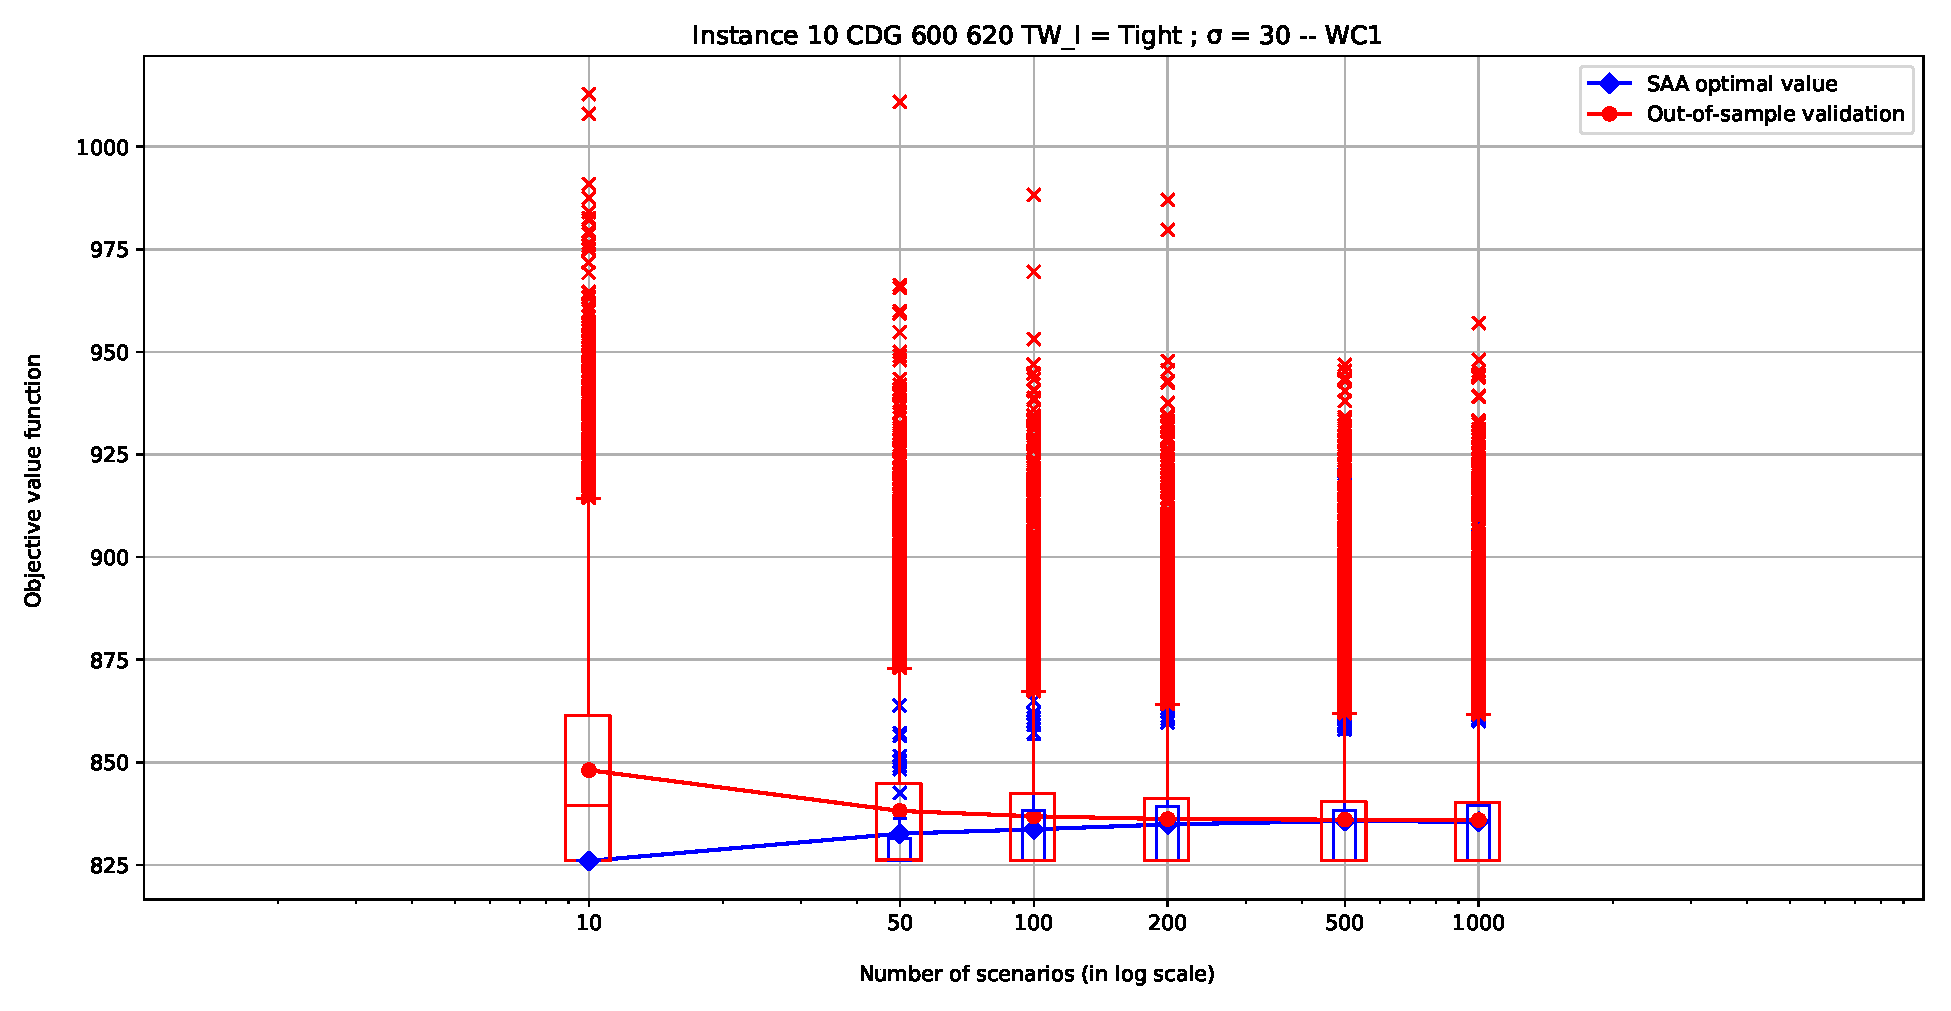
\includegraphics[width=0.56\textwidth]{instance_landing.pdf}
\end{center}

For each number of scenarios $N$: SAA optimal values (blue) and out-of-sample values of the SAA solutions (red). The means move toward each other, from about 826 and 848 for $N = 10$ to about 836 from $N = 200$ on: the two bounds of the previous slides (values read off the figure).

\begin{small}
\textit{Ahmed Khassiba (2020), ``Two-stage stochastic programming for aircraft arrival scheduling under uncertainty'', Ph.D. thesis.}
\end{small}

\end{frame}

\begin{frame}
	\frametitle{SAA for chance constraints}
	
	We consider the problem
	\begin{align*}
		\min_{x \in \mathcal{X}}\ & f(x) \\
		\mbox{s.t. } & P[G(x,\bsxi) \leq 0] \geq 1 - \alpha,
	\end{align*}
	where $G: \rit^n \times \Xi \rightarrow \rit^m$, and $G(x,\xi) \leq 0$ holds componentwise.
	This covers individual ($m = 1$) and joint ($m > 1$) chance constraints.
	
	\mbox{}
	
	With $G_{\max}(x,\xi) := \max_{i = 1,\ldots,m} G_i(x,\xi)$, the constraint fails exactly when $G_{\max}(x,\xi) > 0$, and the problem becomes
	\begin{align*}
		\min_{x \in \mathcal{X}}\ & f(x) \\
		\mbox{s.t. } & P[G_{\max}(x,\bsxi) > 0] \leq \alpha.
	\end{align*}
	
	If this probability has no closed form, we can approximate it by sample average approximation.
	
\end{frame}

\begin{frame}
	\frametitle{SAA of the chance constraint}
	
	With the indicator function of $(0,\infty)$
	\[
	\mathbf{1}_{(0,\infty)}(t) =
	\begin{cases}
		1 & \mbox{if } t > 0,\\
		0 & \mbox{if } t \leq 0,
	\end{cases}
	\]
	we can rewrite the chance constraint as
	\[
	p(x) := \EE\left[ \mathbf{1}_{(0,\infty)} \left( G_{\max}(x, \bsxi) \right) \right] \leq \alpha.
	\]
	
	Let $\xi_1,\ldots,\xi_N$ be an i.i.d. sample of $N$ realizations of $\bsxi$.
	We approximate the chance constraint by
	\[
	\hat{p}_N(x) := \frac{1}{N} \sum_{i = 1}^N \mathbf{1}_{(0,\infty)} \left( G_{\max}(x, \xi_i) \right) \leq \gamma.
	\]
	
\end{frame}

\begin{frame}
	\frametitle{SAA of the chance constraint (cont'd)}
	
	$\hat{p}_N(x)$ is the proportion of draws for which $G_{\max}(x,\xi_i) > 0$.
	The approximate problem is
	\begin{align*}
		\min_{x \in \mathcal{X}}\ & f(x) \\
		\mbox{s.t. } & \hat{p}_N(x) \leq \gamma.
	\end{align*}
	With one binary variable per draw, it is a mixed-integer program (notebook {\tt chance constrained toy example}).
	The level $\gamma$ need not equal $\alpha$:
	\begin{itemize}
	\item
	$\gamma < \alpha$ makes the SAA conservative: its solutions are feasible for the true problem with high probability;
	\item
	$\gamma > \alpha$ enlarges the feasible set of the SAA, whose optimal value is then a lower bound with high probability.
	\end{itemize}
	{\footnotesize J. Luedtke and S. Ahmed (2008), ``A sample approximation approach for optimization with probabilistic constraints'', SIAM Journal on Optimization 19(2), pp. 674--699.}
	
\end{frame}

\begin{frame}
	\frametitle{Theory}
	
	For theoretical justifications, see
	\begin{quote}
		B.K. Pagnoncelli, S. Ahmed, and A. Shapiro (2009), ``Sample Average Approximation Method for Chance
		Constrained Programming: Theory and Applications'', Journal of Optimization Theory and Applications 142 (2), pp. 399--416.
	\end{quote}
	
	\mbox{}
	
	In particular, if $\mathcal{X}$ is compact, $G(\cdot,\xi)$ is continuous for almost every $\xi$, and $P[G_{\max}(x,\bsxi) = 0] = 0$ for every $x \in \mathcal{X}$, then $p$ is continuous on $\mathcal{X}$ and
	\[
	\sup_{x \in \mathcal{X}} |\hat{p}_N(x) - p(x)| \rightarrow 0
	\]
	w.p.1, as $N \rightarrow \infty$: the indicator, bounded by 1, is then continuous at each $x$ for almost every $\xi$, and the ULLN applies.
	
\end{frame}

\begin{frame}
	\frametitle{Convergence}
	
	Assume that  there is an optimal solution $\overline{x}$ of the true problem such that for any $\epsilon > 0$ there is $x \in \mathcal{X}$ with $\| x - \overline{x} \| \leq \epsilon$ and $p(x) < \alpha$.
	
	\mbox{}
	
	\begin{theo}
		Suppose $\gamma = \alpha$, $\mathcal{X}$ compact, $f$ continuous, and $G(\cdot,\xi)$ continuous for almost every $\xi$.
		Then $\hat{v}_N \rightarrow v^*$ and $D(\hat{S}_N,S^*) \rightarrow 0$ almost surely as $N \rightarrow \infty$, where $\hat{v}_N$ and $v^*$ are the optimal values, $\hat{S}_N$ and $S^*$ the sets of optimal solutions, of the approximate and true problems.
	\end{theo}
	
\end{frame}

\begin{frame}
	\frametitle{Application: call centers}
	
	Joint work with Thuy Anh Ta, Tien Mai, Wyean Chan, and Pierre L'Ecuyer.
	The next slides are due to Thuy Anh Ta.
	
	\mbox{}
	
	{\color{red}A call center}: an  office used for receiving or transmitting customer requests by {\color{red}telephone}.
	
	
	\begin{itemize}
		\item A {\color{blue}call} represents a customer and it is classified by {\color{blue}type} ($K$ types). 
		\item Customers are served by {\color{blue}agents}.
		\item Agents sharing a common set of tasks form a {\color{blue}group} of agents ($I$ groups).
		\item A day is divided into {\color{blue}periods} ($P$ periods).
		\item The work schedule of an agent is determined by her {\color{blue}shift} ($Q$ shift configurations).
	\end{itemize}
	
\end{frame}

\begin{frame}{Performance measures}
	\begin{itemize}
		\item{} {\color{blue}{Performance measures} (PM)} assess the quality of service (QoS) and
		efficiency of a call center, e.g., service level (SL), average waiting time (AWT), abandonment ratio, occupancy ratio, etc.
		\item {\color{blue}Service level (SL)}: the percentage of calls that are answered in a defined waiting threshold.
		\item {\color{blue}Average waiting time (AWT)}: the average (or mean) time a customer waited to have a service.
		\item{} QoS can be defined in the long run (expectations), or over a given time period (random variable).
	\end{itemize}
\end{frame}

\begin{frame}{Staffing, Scheduling and Routing}
	\begin{itemize}
		\item{} The objective is to minimize the operating cost of a call center under a set of constraints on certain PMs (SL or AWT).
		\item{} Staffing: deciding the number of agents $y_{i,p}$ of each group for each period in a day.
		\item{} Scheduling:  determining how many agents $x_{i,q}$ to assign to a set of predefined shifts.
		\item{} Routing: determining which agents are allowed to handle the call, and how agents are chosen when several agents are free.
		
	\end{itemize}
	%		\begin{figure}
	%			\includegraphics[width=0.4\linewidth]{figures/planning.pdf}%
	%		\end{figure} 
\end{frame}

\begin{frame}{Modeling a call center}
	\begin{itemize}
		%		\item{} Different types of calls arrive at random and different groups of agents answer these calls
		\item{} The calls arrive according to arbitrary stochastic processes that could be non-stationary (e.g. non-homogeneous Poisson process), and perhaps doubly stochastic (e.g. Poisson--gamma process, whose arrival rate is a gamma random variable).
		\item{} Service times: exponential, log-normal distributions.
		%of calls are traditionally assumed as independent and identically distributed exponential random variables with a constant mean.
		\item{} Delay time,  patience time, etc.
		\item{} With few skills, calls are served in first-come, first-served (FCFS) order, and/or free agents are chosen by the longest-idle-server-first rule.
		\item{} Otherwise, {\color{blue}skill-based routing} may be used to route calls to appropriate agents.
	\end{itemize}
\end{frame}

\begin{frame}{Staffing and scheduling with predictable arrival rates}
	\small
	\[
	\text{SL}(y) = \frac{\mathbb{E}[\text{number of calls answered within } \tau]}{\mathbb{E}[\text{total number of calls}]},
	\]
	and $\text{SL}_{k,p}$, $\text{SL}_p$, $\text{SL}_k$ the same ratio per type and period, per period, per type.

	\textbf{Scheduling problem}	
	\[
	\min {c}^T{x} = \sum_{i=1}^I\sum_{q=1}^Q c_{i,q}x_{i,q}
	\]
	subject to ($A$ maps shifts to periods):
	\begin{equation} \tag{P1}
		\begin{aligned}
			{Ax} &\geq {y} \\
			\text{SL}_{k,p}({y}) &\geq l_{k,p} ~\forall k,p, \\
			\text{SL}_{p}({y}) &\geq l_{p} ~\forall p, \\
			\text{SL}_{k}({y}) &\geq l_{k} ~\forall k, \\
			\text{SL}(y) &\geq l,\\
			{x},{y}&\geq 0 \text{ and integer}  \text{.}\\
		\end{aligned}
	\end{equation}
\end{frame}

\begin{frame}{Staffing and scheduling with predictable arrival rates (cont'd)}
	\textbf{Staffing problem}	
	\[
	\min_y {c'}^T y = \sum_{i=1}^I\sum_{p=1}^P c'_{i,p}y_{i,p}
	\]
	subject to:
	\begin{equation} \tag{P2}
		\begin{aligned}
			\text{SL}_{k,p}({y}) &\geq l_{k,p} ~\forall k,p, \\
			\text{SL}_{p}({y}) &\geq l_{p} ~\forall p, \\
			\text{SL}_{k}({y}) &\geq l_{k} ~\forall k, \\
			\text{SL}(y) &\geq l,\\
			{y}&\geq 0 \text{ and integer}  \text{.}\\
		\end{aligned}
	\end{equation}
\end{frame}

\begin{frame}{Staffing and scheduling}
	
	Over a given period, the service level $S_{k,p}(\tau, y)$ and the average waiting time $W_{k,p}(y)$ are random variables.
	
	The chance-constrained scheduling problem for multiskill call centers is formulated as:
	\[
	\min {c}^T{x} = \sum_{i=1}^I \sum_{q=1}^Q c_{i,q}x_{i,q}
	\]
	subject to:
	\begin{equation} \tag{P3}
		\begin{aligned}
			{Ax} &\geq {y} \\
			\mathbb{P}[S_{k,p}(\tau_{k,p}, {y}) \geq s_{k,p}] &\geq r_{k,p} \text{\qquad{}}  \forall k,p \\
			\mathbb{P}[W_{k,p}(y) \leq w_{k,p}] &\geq  v_{k,p} \text{\qquad{}} \forall k,p\\
			{x}, {y} &\geq 0 \text{ and integer}. \\
		\end{aligned}
	\end{equation}
\end{frame}


\begin{frame}{Sample average approximate problem}
	\[
	\min {c}^T{x} = \sum_{i=1}^I \sum_{q=1}^Q c_{i,q}x_{i,q}
	\]
	subject to:
	\begin{equation} \tag{SAA} \label{s1}
		\begin{array}{ll}
			{Ax} &\geq {y} \\
			\displaystyle \frac{1}{N} \sum_{d=1}^N\mathbb{I}[\hat{S}_{N, k,p}^d(\tau_{k,p}, {y}) \geq s_{k,p}] &\geq r_{k,p} \text{\qquad{}}\forall k,p\\
			\displaystyle \frac{1}{N}\sum_{d=1}^N\mathbb{I}[\hat{W}_{N,k,p}^d({y}) \leq w_{k,p}]&\geq v_{k,p} \text{\qquad{}}\forall k,p\\
			{x}, {y} &\geq 0 \text{ and integer}  \text{ .}\\
		\end{array}
	\end{equation}
	Under some specific conditions, the optimal value and the set of optimal solutions of the SAA problem converge to those of the true problem  with probability one as $N$ approaches infinity. 
\end{frame}

\begin{frame}{Arrival-rate uncertainty: two-stage staffing}
	
	Arrival rates are not known in advance, and their forecasts improve as the day approaches. For a single period:
	\begin{itemize}
		\item
		{\blue Stage 1} (days ahead): staffing $x \in \mathbb{N}^I$, at cost $c^Tx$, under a prior forecast of the arrival rates;
		\item
		{\blue Stage 2} (a few hours ahead): an updated forecast $\xi$ is observed; $r^+$ agents can be added at unit cost $c^+ > c$, and $r^- \leq x$ removed, refunded $c^- < c$; the staffing becomes $z(\xi) = x + r^+ - r^-$;
		\item
		the service level $S_k(z)$ of call type $k$ over the period is a random variable ($k = 0$: all calls).
	\end{itemize}
	\begin{align*}
	& \min_{x} \ c^Tx + \EE_{\xi}[Q(x,\xi)], \\
	& Q(x,\xi) = \min_{r^+, r^-} \ (c^+)^Tr^+ - (c^-)^Tr^- \ \ \text{s.t.} \ \ P[S_k(z(\xi)) \geq l_k \mid \xi] \geq 1 - \delta_k\ \forall k.
	\end{align*}
	A two-stage program (deck~03) with integer recourse and chance constraints (deck~05) in the second stage.
	
\end{frame}

\begin{frame}{Nested SAA}
	\small
	
	The probabilities have no closed form: they are estimated by simulation, inside each scenario.
	\begin{itemize}
		\item
		{\blue Outer sample}: $N$ scenarios $\xi_1, \ldots, \xi_N$ of the forecast update. {\blue Inner sample}: for each $\xi_n$, $M$ simulations of the period, conditional on $\xi_n$; each chance constraint becomes
		\[
		\hat{g}_{k,M}(z_n; \xi_n) := \frac{1}{M} \sum_{m=1}^M \mathbb{I}\left[\hat{S}_k^m(z_n; \xi_n) \geq l_k\right] \geq 1 - \delta_k,
		\]
		the indicator SAA of the previous slides, once per scenario.
		\item
		{\blue SAA}: $\min \ c^Tx + \frac{1}{N} \sum_{n=1}^N \left[ (c^+)^Tr_n^+ - (c^-)^Tr_n^- \right]$, with $z_n = x + r_n^+ - r_n^-$.
	\end{itemize}
	
	{\blue Consistency}: optimal values and solutions converge w.p.1 when $N$ and $M$ grow together; under further assumptions, the probability of an incorrect solution decays exponentially (Ta, Mai, Bastin, L'Ecuyer, 2021).
	
	{\blue Solution}: linear cuts from simulated subgradients replace the chance constraints (Chan et al., 2016); L-shaped decomposition over the scenarios (deck~04; Ta, Chan, Bastin, L'Ecuyer, 2021).
	
\end{frame}

\begin{frame}{Consistency in practice}
	
	Small center: $K = 2$ call types, $I = 2$ agent groups.
	For each $M = N$, 20 independent SAA problems are solved; each solution is compared, out of sample, with the optimal solution of an independent {\blue validation} SAA with $M = N = 1000$. The table counts the SAA solutions that are optimal for the validation problem.
	
	\begin{center}
		\begin{tabular}{l|ccccccc}
			$M = N$ & 50 & 100 & 200 & 400 & 600 & 800 & 1000 \\
			\hline
			optimal (out of 20) & 0 & 5 & 0 & 1 & 8 & 15 & 20
		\end{tabular}
	\end{center}
	
	\begin{itemize}
		\item
		The feasible set is finite: once the samples are large enough, the SAA returns {\red exactly} the optimal solution. At $M = N = 1000$, the 20 SAA solutions coincide.
		\item
		With 20 replications, the count is noisy at small sizes; the estimated gaps decrease steadily.
	\end{itemize}
	
	{\footnotesize Counts read off Figure 1 of Ta, Mai, Bastin, and L'Ecuyer (2021).}
	
\end{frame}

\begin{frame}{Out-of-sample validation in practice}
	
	Medium center: $K = 6$ call types, $I = 8$ groups, $M = 1000$ simulations per scenario; targets $(1-\delta_k, 1-\delta_0) = (0.80, 0.85)$; $c^+ = 1.1c$, $c^- = 0.9c$. Each first-stage solution is evaluated on 100 independent scenarios.
	
	\begin{center}
		\begin{tabular}{c|cc|cc}
			& \multicolumn{2}{c|}{Cost (L-shaped)} & \multicolumn{2}{c}{Total CPU time (hours)} \\
			$N$ & in-sample & out-of-sample & L-shaped & direct MIP \\
			\hline
			20 & 180.10 & 187.41 & 1.54 & 2.67 \\
			50 & 177.43 & 184.15 & 1.84 & 5.48 \\
			70 & 175.31 & 183.32 & 3.93 & 10.44
		\end{tabular}
	\end{center}
	
	\begin{itemize}
		\item
		The in-sample cost is {\red optimistic}, as the bias of $v_N$ predicts: in 15 of the 18 configurations of the paper.
		\item
		The out-of-sample cost decreases with $N$: larger samples give better first-stage decisions.
		\item
		Decomposition divides the computing time by about 2 to 3.
	\end{itemize}
	
	{\footnotesize Ta, Chan, Bastin, and L'Ecuyer (2021), Table 3 (case R3).}
	
\end{frame}

\begin{frame}{Application: references}
	
	\begin{itemize}
		\item
		W. Chan, T. A. Ta, P. L'Ecuyer, and F. Bastin (2016), ``Two-stage chance-constrained staffing with agent recourse for multi-skill call centers'', {\sl Proceedings of the 2016 Winter Simulation Conference}, pp. 3189--3200.
		\item
		T. A. Ta, T. Mai, F. Bastin, and P. L'Ecuyer (2021), ``On a multistage discrete stochastic optimization problem with stochastic constraints and nested sampling'', {\sl Mathematical Programming} 190(1--2), pp. 1--37.
		\item
		T. A. Ta, W. Chan, F. Bastin, and P. L'Ecuyer (2021), ``A simulation-based decomposition approach for two-stage staffing optimization in call centers under arrival rate uncertainty'', {\sl European Journal of Operational Research} 293(3), pp. 966--979.
	\end{itemize}
	
\end{frame}

\begin{frame}
\frametitle{Further reading}
\footnotesize

\begin{itemize}
\item
A. Shapiro, D. Dentcheva, and A. Ruszczy\'nski, {\sl Lectures on Stochastic Programming: Modeling and Theory}, 3rd edition, SIAM, 2021, Chapter~5 (first edition, 2009, freely available).
\item
T. Homem-de-Mello and G. Bayraksan (2014), ``Monte Carlo sampling-based methods for stochastic optimization'', {\sl Surveys in Operations Research and Management Science} 19(1), pp. 56--85.
\item
A. J. Kleywegt, A. Shapiro, and T. Homem-de-Mello (2002), ``The sample average approximation method for stochastic discrete optimization'', {\sl SIAM Journal on Optimization} 12(2), pp. 479--502.
\item
W.-K. Mak, D. P. Morton, and R. K. Wood (1999), ``Monte Carlo bounding techniques for determining solution quality in stochastic programs'', {\sl Operations Research Letters} 24(1--2), pp. 47--56.
\item
F. Bastin, C. Cirillo, and Ph. L. Toint (2006), ``Convergence theory for nonconvex stochastic programming with an application to mixed logit'', {\sl Mathematical Programming} 108(2--3), pp. 207--234.
\item
B. K. Pagnoncelli, S. Ahmed, and A. Shapiro (2009), ``Sample average approximation method for chance constrained programming: theory and applications'', {\sl Journal of Optimization Theory and Applications} 142(2), pp. 399--416.
\end{itemize}

\end{frame}

\end{document}